% mn2esample.tex
%
% v2.1 released 22nd May 2002 (G. Hutton)
%
% The mnsample.tex file has been amended to highlight
% the proper use of LaTeX2e code with the class file
% and using natbib cross-referencing. These changes
% do not reflect the original paper by A. V. Raveendran.
%
% Previous versions of this sample document were
% compatible with the LaTeX 2.09 style file mn.sty
% v1.2 released 5th September 1994 (M. Reed)
% v1.1 released 18th July 1994
% v1.0 released 28th January 1994

\documentclass[useAMS,usenatbib]{mn2e}
%FAG added header file to contain macros

\usepackage{amsmath}
\usepackage{bm}
\usepackage{mathtools}
\usepackage{graphicx,subfigure}
\usepackage{caption}
\usepackage{varioref}
\usepackage{float}
\restylefloat{table}
% model labels
  \newcommand{\Op}{{WSWa}}
  \newcommand{\OpH}{{WSWah}}
  \newcommand{\WSWa}{{WSWb}}
  \newcommand{\Omp}{{\Omega}}
  \newcommand{\Ompa}{{\mathrm{B}1\rm{\Omega} }}
  \newcommand{\Ompb}{{\mathrm{B}1\rm{\Omega}\rm{O}}}
  \newcommand{\Ompc}{{\mathrm{B}1\rm{\Omega}\rm{SN}}}
  \newcommand{\Ompd}{{\mathrm{B}2\rm{\Omega}}}
  \newcommand{\Ompe}{{\mathrm{B}1\rm{\Omega}\rm{Sh}}}
  \newcommand{\Omph}{{\mathrm{H}1\rm{\Omega}}}
  \newcommand{\HDI}{{(HDI)}} %update with {{\cite{HDI}}} once submitted and bib
% physical quantities
  \newcommand{\cm}{\,{\rm cm}}
  \newcommand{\mm}{\,{\rm mm}}
  \newcommand{\cmcube}{\,{\rm cm^{-3}}}
  \newcommand{\dyn}{\,{\rm dyn}}
  \newcommand{\erg}{\,{\rm erg}}
  \newcommand{\g}{\,{\rm g}}
  \newcommand{\Jy}{\,{\rm Jy}}
  \newcommand{\Jyb}{\,{\rm Jy/beam}}
  \newcommand{\km}{\,{\rm km}}
  \newcommand{\kms}{\,{\rm km\,s^{-1}}}
  \newcommand{\mJy}{\,{\rm mJy}}
  \newcommand{\mJyb}{\,{\rm mJy/beam}}
  \newcommand{\K}{\,{\rm K}}
  \newcommand{\kpc}{\,{\rm kpc}}
  \newcommand{\pc}{\,{\rm pc}}
  \newcommand{\Mpc}{\,{\rm Mpc}}
  \newcommand{\Myr}{\,{\rm Myr}}
  \newcommand{\Gyr}{\,{\rm Gyr}}
% tags
  \newcommand{\str}{\mathcal{D}}
  \newcommand{\corr}{\mathcal{C}}
  \newcommand{\lcorr}{\mathcal{L}}
  \newcommand{\turb}{_{\rm turb}}     			%turbulent
% maths symbols
  \newcommand\mean[1]{\overline{#1}}         %ensemnle average
  \newcommand{\vect}[1]{{{\mbox{\boldmath $#1$}}}}%also makes bold Greek letters
% Journals
  \newcommand{\HD}{{Paper\,I}} 				%Paper I
  \newcommand{\MHD}{{Paper\,II}} 				%Paper I
  \newcommand{\aap}{{A{\&}A}}
  \newcommand{\an}{{Astron.\ Nachr.}}
  \newcommand{\apj}{{ApJ}}
  \newcommand{\apjl}{{ApJL}}
  \newcommand{\apjs}{{ApJS}}
  \newcommand{\mnras}{{MNRAS}}
  \newcommand{\aj}{{AJ}}
  \newcommand{\nat}{{Nature}}
  \newcommand{\ssr}{{SSRv}}
  \newcommand{\araa}{ARA\&A}
  \newcommand{\rmp}{{Rev.\ Mod.\ Phys.}}
  \newcommand{\solphys}{{SoPh}}
  \newcommand{\physrep}{{Phys.\ Rep.}}
  \newcommand{\jfm}{{J.\ Fluid Mech.}}    

%\usepackage{amsmath}
%\usepackage{bm}
%\usepackage{mathtools}
%\usepackage{graphicx,subfigure}
%\usepackage{caption}
%\usepackage{varioref}
%\usepackage{float}
%\restylefloat{table}
% If your system does not have the AMS fonts version 2.0 installed, then
% remove the useAMS option.
%
% useAMS allows you to obtain upright Greek characters.
% e.g. \umu, \upi etc.  See the section on "Upright Greek characters" in
% this guide for further information.
%
% If you are using AMS 2.0 fonts, bold math letters/symbols are available
% at a larger range of sizes for NFSS release 1 and 2 (using \boldmath or
% preferably \bmath).
%
% The usenatbib command allows the use of Patrick Daly's natbib.sty for
% cross-referencing.
%
% If you wish to typeset the paper in Times font (if you do not have the
% PostScript Type 1 Computer Modern fonts you will need to do this to get
% smoother fonts in a PDF file) then uncomment the next line
% \usepackage{Times}

%%%%% AUTHORS - PLACE YOUR OWN MACROS HERE %%%%%


%%%%%%%%%%%%%%%%%%%%%%%%%%%%%%%%%%%%%%%%%%%%%%%%

\title[Statistical Geometry of the turbulent multi-phase ISM - I. Field lines]{Statistical Geometry of the turbulent ISM - I. Field lines}
\author[C. C.~Evirgen, A.~Shukurov, F.A. Gent and A.~Fletcher]{C.C.~Evirgen$^{1}$\thanks{E-mail:
c.c.evirgen@newcastle.ac.uk (CCE); anvar.shukurov@newcastle.ac.uk (AS); 
f.gent@shef.ac.uk (FAG); andrew.fletcher@newcastle.ac.uk (AF)}, A.~Shukurov$^{1}$, F.A.~Gent$^{2}$ and A.~Fletcher$^{1}$.\\%$^{2}$\footnotemark[1]\thanks{This file has been amended to
%highlight the proper use of \LaTeXe\ code with the class file.
%These changes are for illustrative purposes and do not reflect the
%original paper by A. V. Raveendran.}\\
$^{1}$School of Mathematics and Statistics, Newcastle University,
Newcastle upon Tyne, UK, NE1 7RU\\
$^{2}$SP$^{\,2}$\!RC, School of Mathematics and Statistics, University of Sheffield, 
Sheffield, UK, S3 7RH}
\begin{document}
\newcommand{\bvec}[1]{\boldsymbol{#1}}
\newcommand{\avg}[1]{\left<\bvec{#1}\right>_{l}}
\date{Accepted -. Received -; in original form -}

\pagerange{\pageref{firstpage}--\pageref{lastpage}} \pubyear{2014}

\maketitle

\label{firstpage}

\begin{abstract}
Abstract to be left until the end. Words, words and more words to follow but first we need a paper. There will be methods, keywords and results hinted at here. 
\end{abstract}

\begin{keywords}
circumstellar matter -- infrared: stars.
\end{keywords}

\section{Introduction}
%FAG rephrase
%The results presented in this paper are based on simulations of the multiphase interstellar medium (ISM) by Gent \textsl{et al} in \citep{GSFSM13} and \citep{GSSFM13}, %further referencing to Paper I & II needed here.
The results presented in this paper are based on simulations of the multiphase 
interstellar medium (ISM) reported in \citet{GSFSM13} and \citet{GSSFM13}, %further referencing to Paper I & II needed here.
subsequently referred to as \HD\, and \MHD, respectively.
%end FAG
%FAG rephrase
In particular we consider a model, identified as B1$\Omega$s in \MHD.
Supernova(SN)-driven turbulence is applied to ISM in a section of a spiral
galaxy differentially rotating, stratified about the galactic disk and subject
to, radiative cooling, photoelectric heating and other transport processes.
The rate and distribution of SN explosions, gravity and angular momentum are 
consistent with observational parameters for the solar neighbourhood.
A nano Gauss seed magnetic field is applied and amplified by dynamo until it
saturates with a mean magnetic stength of a few micro Gauss, remarkably 
consistent with observed estimates for the Milky Way.

Models of the magnetized ISM \citep{Heitsch01,M-LBKA05} 
%FAG maybe also include Henley et al 2015 end FAG
have explored the 
effects of magnetic field on the localized ISM, including the fluctuation 
dynamo, but without the effects of stratification and the large scale 
structure induced by the differential rotation of the disk.
Large scale structure in the stratified ISM has been investigated by
\citet{AB05a}, but without differential rotation the dynamo to grow the field
to full strength is absent, so an imposed field is applied. 
\citet{Hanasz05,Dobbs08} and \citet{Hanasz09} apply magnetic fields to global 
disk models, including a dynamo, but due to numerical constraints must limit or 
exclude vertical stratification and multi-phase gas composition.
\citet{Korpi99a} and \cite{Gressel08} conducted earlier simulations with the
same approach as described here, but with lower resolution and higher 
diffusion were unable to follow the dynamo through to saturation.
The advantage of the results from \MHD\ is that the magnetic field produced
is not imposed, but evolves dynamically under realistic physical processes
governing the formation of the thermo-hydrodynamic structure of the ISM.
From this point of view it is of great value for appreciating the 
multi-phase structure of the magnetized ISM and for comparison with observation.

%focusing on the the B1$\Omega$s model of the ISM. This model features supernova(SN)-driven turbulence with gravity, differential rotation, SN explosions (SNe), radiative cooling, photoelectric heating and other transport processes, where the dynamo is in a kinematic statistically-steady state \citep{GSFSM13,GSSFM13}.\\
%end FAG
A snapshot of the ISM at approximately $t=1.4$ Gyr is used. Its characteristics, in terms of the fractional volumes of the phases, is representative of the steady-state phase of the dynamo. In addition, there are two potential SN remnants, which provide isolated structures of hot gas. This enhances the illustration of the effect that hot gas has on the mean magnetic field. 

The multi-phase structure is defined in terms of temperature and density. However, an equivalent definition is given in terms of entropy, which has an explicit defintion linking density and temperature \citep{Gent12}. The cold, warm and hot phases are defined by the entropy ranges, $s\leq3.7\cdot10^8$, $3.7\cdot10^8<s<23.2\cdot10^8$ and $s>23.2\cdot10^8$ erg g$^{-1}$ K$^{-1}$, respectively. 
\section{The mean magnetic field}
When considering the mean-field decomposition of the magnetic field, the notation used by \citep{GSSFM13} is adopted.
Volume averaging with a Gaussian kernel, $G_{l}(\bvec{x}-\bvec{x}')$ is used to decompose the magnetic field, $\bvec{B}$, into mean (large-scale), $\bvec{B}_{l}$ and random (small-scale), $\bvec{b}_{l}$, fields. The decomposition is given by 
\begin{equation}
\bvec{B} = \bvec{B}_{l}+\bvec{b}_{l},\qquad \bvec{B}_{l} = \avg{B}. \label{decomp} 
\end{equation}
Gaussian smoothing of the magnetic field with kernel size $l$ is represented by
\begin{align}
\avg{B}&=\int_{V}\bvec{B}(\bvec{x}')G_{l}(\bvec{x}-\bvec{x}')d^{3}\bvec{x}',\\
G_{l}(\bvec{x})&=(2\pi l^2)^{-3/2}\exp[-\bvec{x}/(2l^2)],\nonumber
\label{gauss}
\end{align} 
where $l\approx50$pc is half the integral scale of random motions \citep{GSSFM13}. This value is adopted for this paper based on the justification given in \citep{gent2}.  Preliminary analysis does not show significant sensitivity of the mean or random field to variations in $l$ within the range $0<l<100$pc. However, future work will consider analysis of isolated structures in the ISM. A more detailed analysis of length and correlation scales will be carried out. However, the current definition, $l=50$pc, is sufficient for the purposes of this paper. 
%\begin{table*}
 %\centering
 %\begin{minipage}{140mm}
  %\caption{Data on the RV Tauri stars detected by {\it IRAS}.}
  %\begin{tabular}{@{}llrrrrlrlr@{}}
  %\hline
  % Name     &            & \multicolumn{4}{c}{Flux density (Jy)%
 %\footnote{Observed by {\em IRAS}.}}\\
 % Variable & {\it IRAS} & 12$\,\umu$m & 25$\,\umu$m & 60$\,\umu$m
 %    & 100$\,\umu$m & Sp. & Period & Light- & $T_0\,(\rmn{K})$ \\
 %       &  &  &  &  &  & group & (d) & curve \\
 %       &  &  &  &  &  &       &     & type  \\
 %\hline
 %TW Cam & 04166$+$5719 & 8.27 & 5.62 & 1.82 & $<$1.73 & A & 85.6 & a & 555 \\
 %RV Tau & 04440$+$2605 & 22.53 & 18.08 & 6.40 & 2.52 & A & 78.9 & b & 460 \\
%\hline
%\end{tabular}
%\end{minipage}
%\end{table*}
%FAG added section from thesis -- to be edited
%-----------------------------------------------------------------------------
\section{Three-phase structure of the Field}\label{sect:3BB}
%-----------------------------------------------------------------------------

  The total volume probability distributions for gas number density $n$, 
  temperature $T$ and thermal pressure $p$ are displayed in Fig.~\ref{fig:pdfm}
  from Models~$\Ompa$ (black, solid) and $\Omph$ (blue, dashed). 
%  Note that Model~$\Omph$ includes the correction to the SN distribution,
%  which stabilises the disc against unphysical cyclic oscillations, although
%  it is still subject to natural random vertical fluctuations.
%  Hence the mean density in the SN active region remains consistently higher
%  than in Model~\Op.
%-----------------------------------------------------------------------------
  \begin{figure}
  \centering
  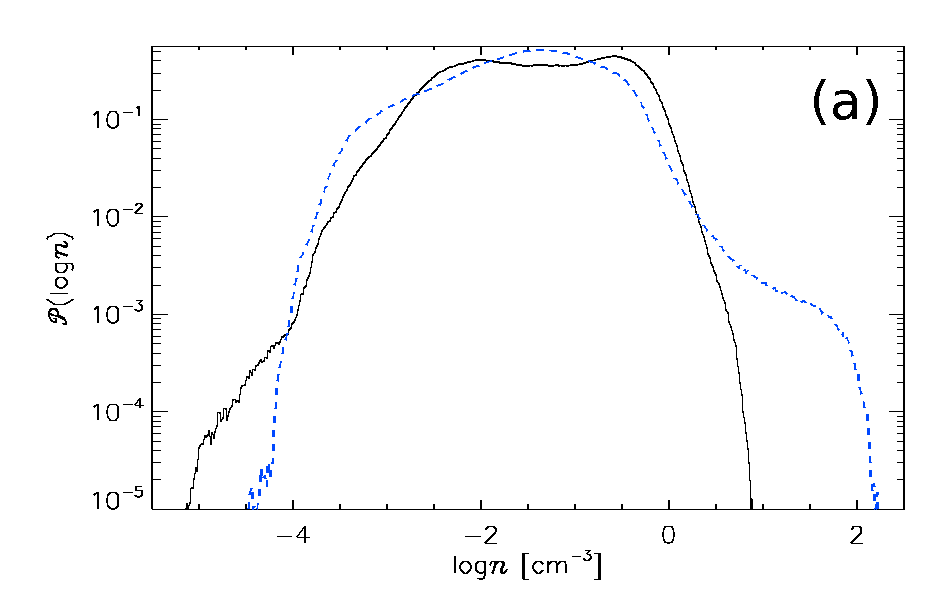
\includegraphics[width=0.9\columnwidth,clip=true,trim=0 0 0 9mm]{fig/o1pr_rpdf.png}
  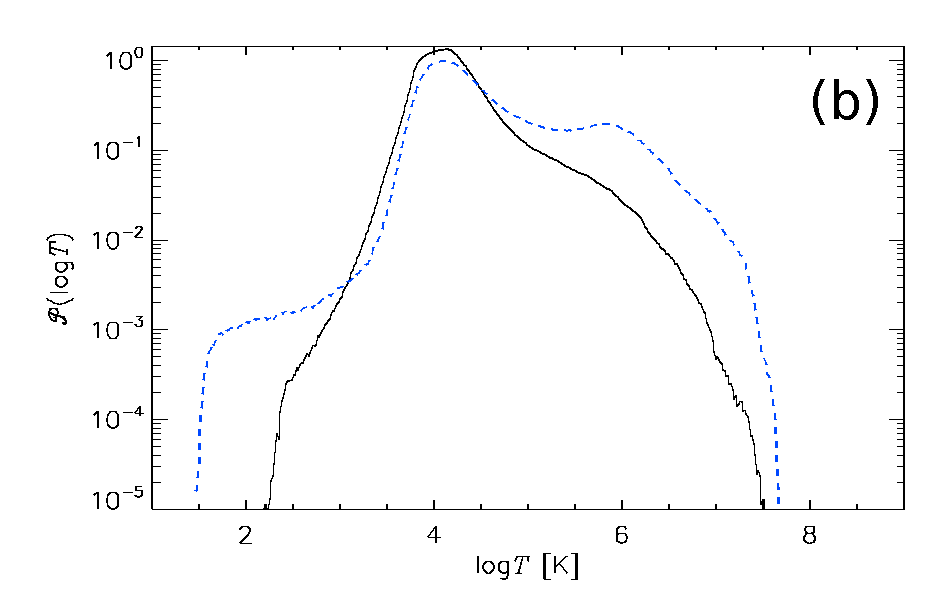
\includegraphics[width=0.9\columnwidth,clip=true,trim=0 0 0 9mm]{fig/o1pr_tpdf.png}
  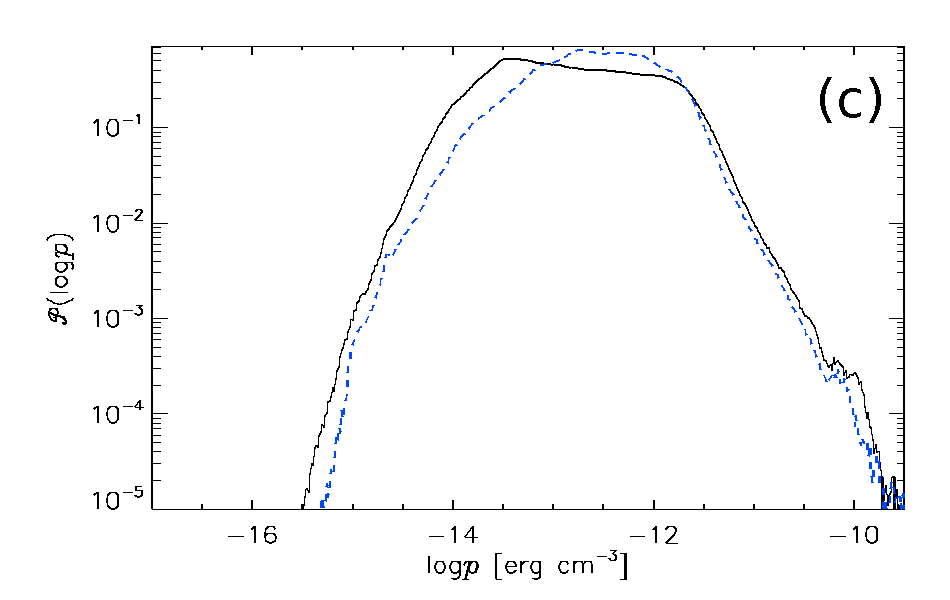
\includegraphics[width=0.9\columnwidth,clip=true,trim=0 0 0 9mm]{fig/o1pr_ppdf.png}
    \caption[Total volume probability distributions for Model~$\Ompa$ and $\Omph$]{
  Volume weighted probability distributions of gas number
  density~{\textbf{(a)}}, temperature~{\textbf{(b)}} and thermal
  pressure~{\textbf{(c)}} for  models {$\Omph$} (black, solid) and
  {$\Ompa$} (blue, dashed) for the total numerical domain $|z|\le1.12\kpc$.
    \label{fig:pdfm}}
  \end{figure}
%-----------------------------------------------------------------------------
  A three phase temperature distribution is visible for Model~$\Omph$ (HD)
  model in Fig.~\ref{fig:pdfm}b, while less apparent for Model~$\Ompa$ (MHD),
  with a significantly narrower range of temperatures.
  The bulk of the density distributions (a) are quite similar between the 
  HD and MHD model, except that the high densities are not as well resolved in
  the MHD model.
  The thermal pressure distributions are very similar, but with the HD modal
  pressure approximately one third the MHD modal pressure. 
  \footnote{FAG: I think these plots are averages of several snapshots in the 
  kinematic dynamo -- need to check -- while the analysis elsewhere is on the 
  saturated field}
  Even with a relatively weak magnetic field, there is significantly increased
  stiffness to the ISM, which restricts transport of the hot gas away from the
  disk (FAG: Kompaneets?), and may also act as a break on the supersonic
  flows, reducing the material collected in the snowplough phase of the SN and
  hence less cold gas resolved in the model (FAG: cite?)
%-----------------------------------------------------------------------------
  \begin{figure}
  \centering
  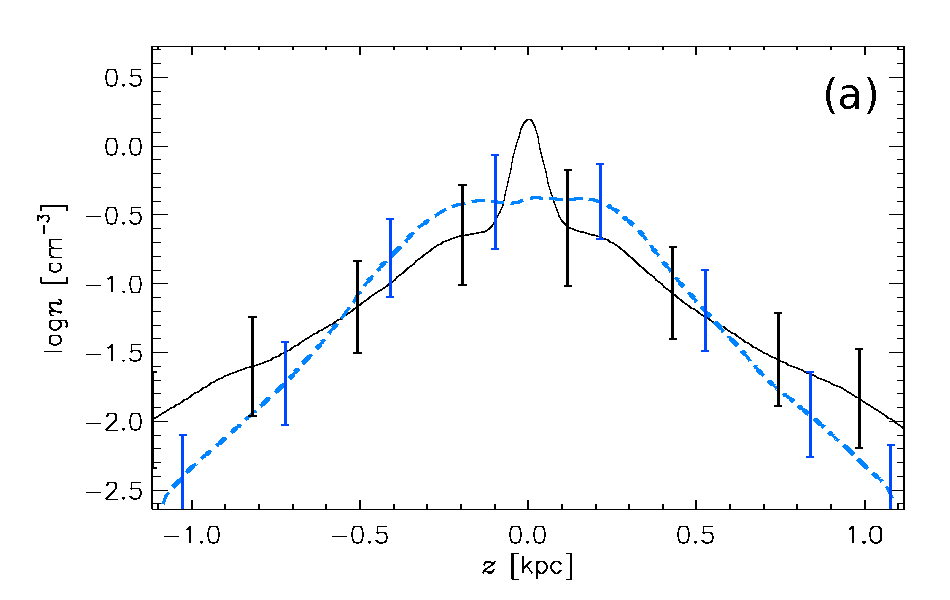
\includegraphics[width=0.9\columnwidth]{fig/zrhom.png}
  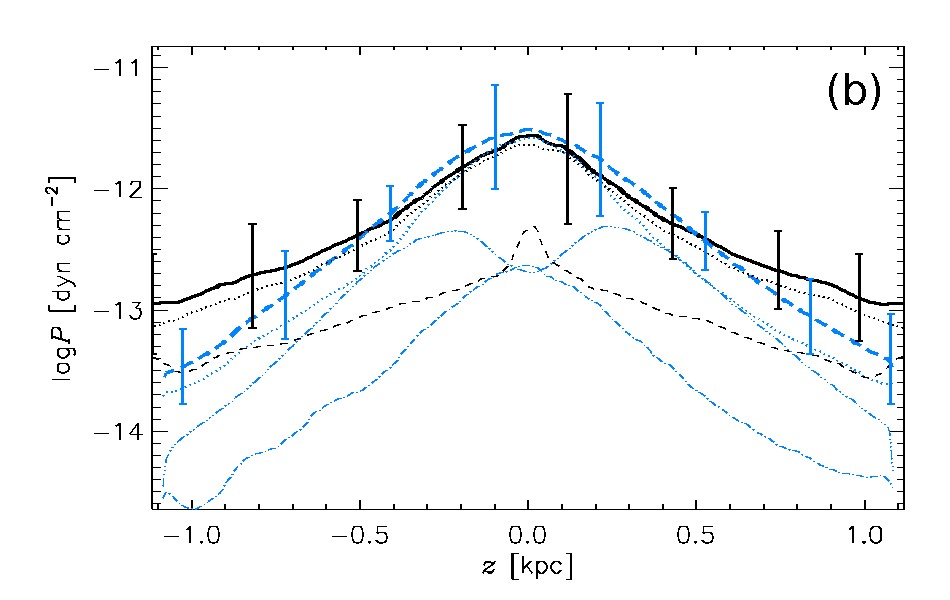
\includegraphics[width=0.9\columnwidth]{fig/zrppm.png}
    \caption[Horizontal averages of $n$ and $P$ for Model~$\Ompa$ and $\Omph$]{
  Horizontal averages of gas number density, $\mean{n}(z)$ {\textbf{(a)}}, and
  total pressure, $\mean{P}(z)$ {\textbf{(b)}}, for Model~{$\Ompa$} (solid,
  black), and Model~{$\Omph$} (dashed, blue). 
  Each are time-averaged using eleven snapshots respectively, spanning 
  100\Myr.
  The vertical lines indicate standard deviation within each horizontal slice.
  The thermal $\mean{p}(z)$ (dotted) and ram $\mean{p}\turb(z)$ (fine dashed)
  pressures are also plotted {\textbf{(b)}}.
%  For Model~{\OpH} the magnetic pressure $\mean{p}_B$ is also plotted (fine, 
%  dash-3dotted).
    \label{fig:zrhom}
            }
  \end{figure}
%-----------------------------------------------------------------------------

%  As discussed in Section~\ref{subsect:params} the stability of the disc
%  reduces the effectiveness of the SNe to generate and circulate hot gas, in
%  the absence of SN clustering. 
%  Hence Model~$\Omph$ has a slightly thicker disc, with less hot gas than 
%  Model~\Op.
  The effect of the magnetic pressure in Model~$\Ompa$ is to 
  expand the thick disc even further and this is illustrated in 
  Fig.~\ref{fig:zrhom}a, where the horizontal averages of gas number density
  $n(z)$ are plotted against $z$ for both models. 
  The strong peak in the density at the mid-plane is evident for Model~$\Omph$
  (black, solid), while for Model~$\Ompa$ (blue, dashed) there is a broad
  plateau in the density, extending to $|z|\simeq300\pc$, where the mean 
  magnetic field is strongest.
  
%-----------------------------------------------------------------------------
  \begin{figure}
  \centering
  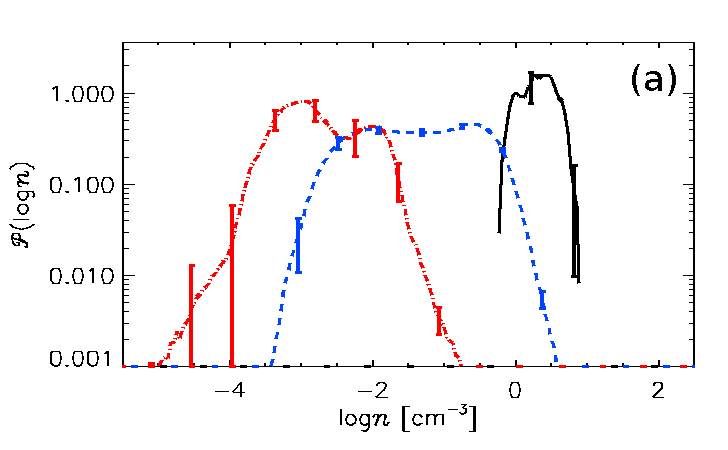
\includegraphics[width=0.9\linewidth]{fig/o1pr_npdf3s.png}  
  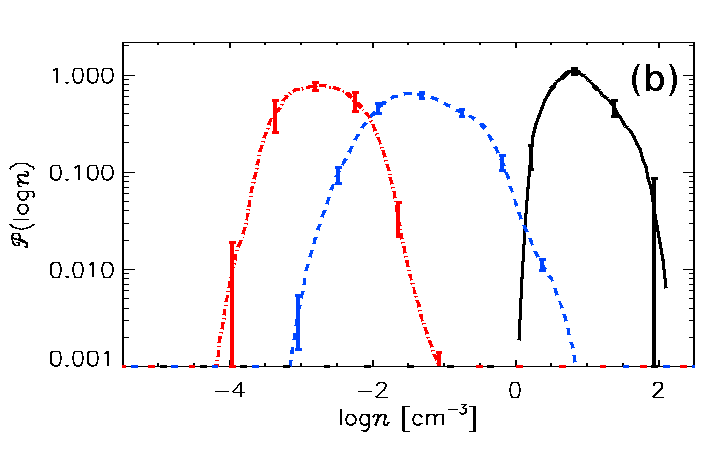
\includegraphics[width=0.9\linewidth]{fig/o1ph_npdf3s.png}\\  
  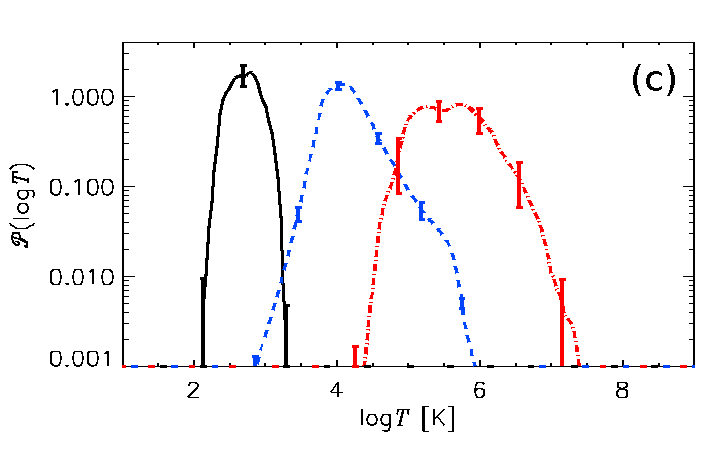
\includegraphics[width=0.9\linewidth]{fig/o1pr_tpdf3s.png}
  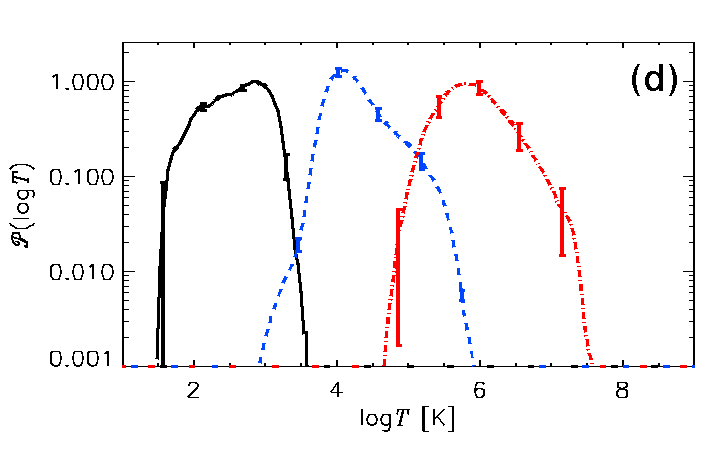
\includegraphics[width=0.9\linewidth]{fig/o1ph_tpdf3s.png}  
    \caption[Probability distributions by phase for $n$ and $T$]{
  Probability distributions by phase: cold (blue, dashed), warm (black, solid)
  and hot (red, dash-dotted) for gas number density ($n$ {\textbf{(a), (b)}})
  and temperature ($T$ {\textbf{(c), (d)}}) 
  for Model~$\Ompa$ ({\textbf{(a), (c)}}) and Model~$\Omph$
  ({\textbf{(b), (d)}}).
%  Data are averaged over 100\,Myr using eleven snapshots. 
  95\% confidence intervals for temporal deviation are shown as error bars.   
  \label{fig:npdf3s}
    }
  \end{figure}
%-----------------------------------------------------------------------------

  The horizontal averages of the pressure are plotted in Fig.~\ref{fig:zrhom}b
  for both models. 
  There is a strong peak at the mid-plane in the turbulent pressure for the HD
  model (black, dashed), but a much weaker profile for the MHD model (blue,
  dash-dotted). 
  There are two peaks in the magnetic pressure (blue, dash-3dotted) near 
  $|z|\simeq200\pc$, which supports the extended density profile.
  Another possible effect, which might constrain the circulation of the hot
  gas, and hence enhance the pressure at the mid-plane, is the strong 
  horizontal orientation of the field.
  The periodic boundary conditions
  exclude a non-zero vertical component to the mean field, so the magnetic
  tension predominantly acts against the vertical flows.
  Some understanding of the multi-phase structure of the magnetised ISM is
  still possible from these models, but the extreme temperatures and densities
  are significantly under represented.
  To improve this in future work it will be desirable to allow unrestricted 
  evolution of vertical field and to apply realistic clustering of the 
  SNe to generate more supperbubbles (composite multiple SN remnants forming a
  single superstructure) or chimneys (plumes venting hot gas from the disc 
  towards the halo).

  Results for separation of the ISM into three phases using the method 
  detailed in \cite[][Ch. 5.3]{Gent12} are shown for Models~$\Ompa$ and
  $\Omph$ in Fig~\ref{fig:npdf3s} with total volume probability distributions.
  The phases are defined using entropy $s$ such that for cold 
  $s<4.4\cdot10^{8}\erg \g^{-1}\K^{-1}$ and hot 
  $s>23.2\cdot10^{8}\erg \g^{-1}\K^{-1}$ with warm in between.
  Apart from the higher densities for the cold phase with the HD model (panel 
  b), 
  anticipated by the volume distributions (Fig.~\ref{fig:pdfm}), the warm and
  hot distributions for the MHD density (panel a) are broad, with a bimodal 
  structure to the hot gas. 
  The distributions for the warm gas (panels c and d) are very similar and for
  the cold (hot) distributions the MHD model does not extend to as low (high)
  temperatures. 
  
%-----------------------------------------------------------------------------
  \begin{figure}
  \centering
  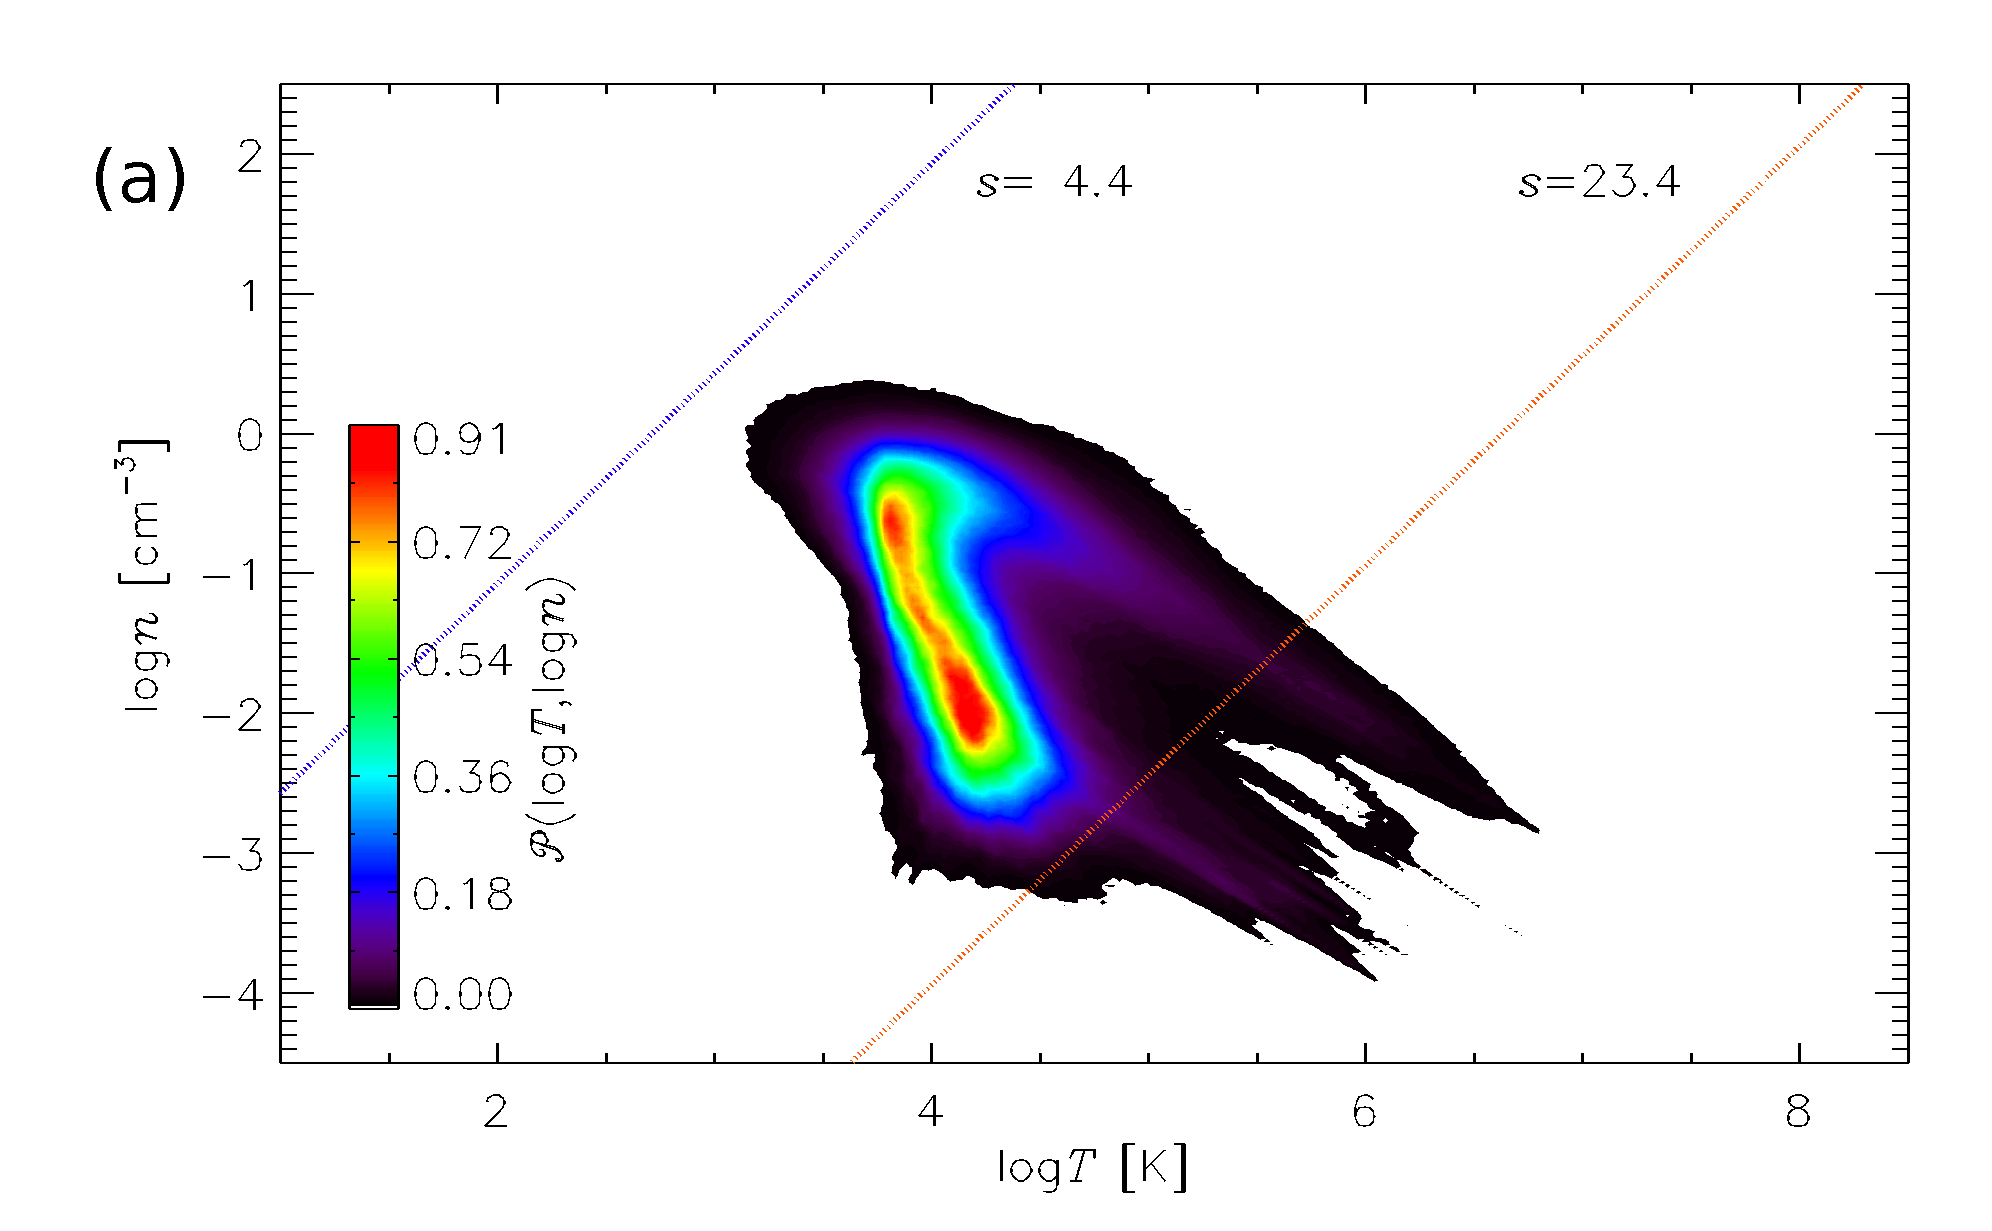
\includegraphics[width=0.9\linewidth]{fig/o1pr_pdf2dtn.png}  
  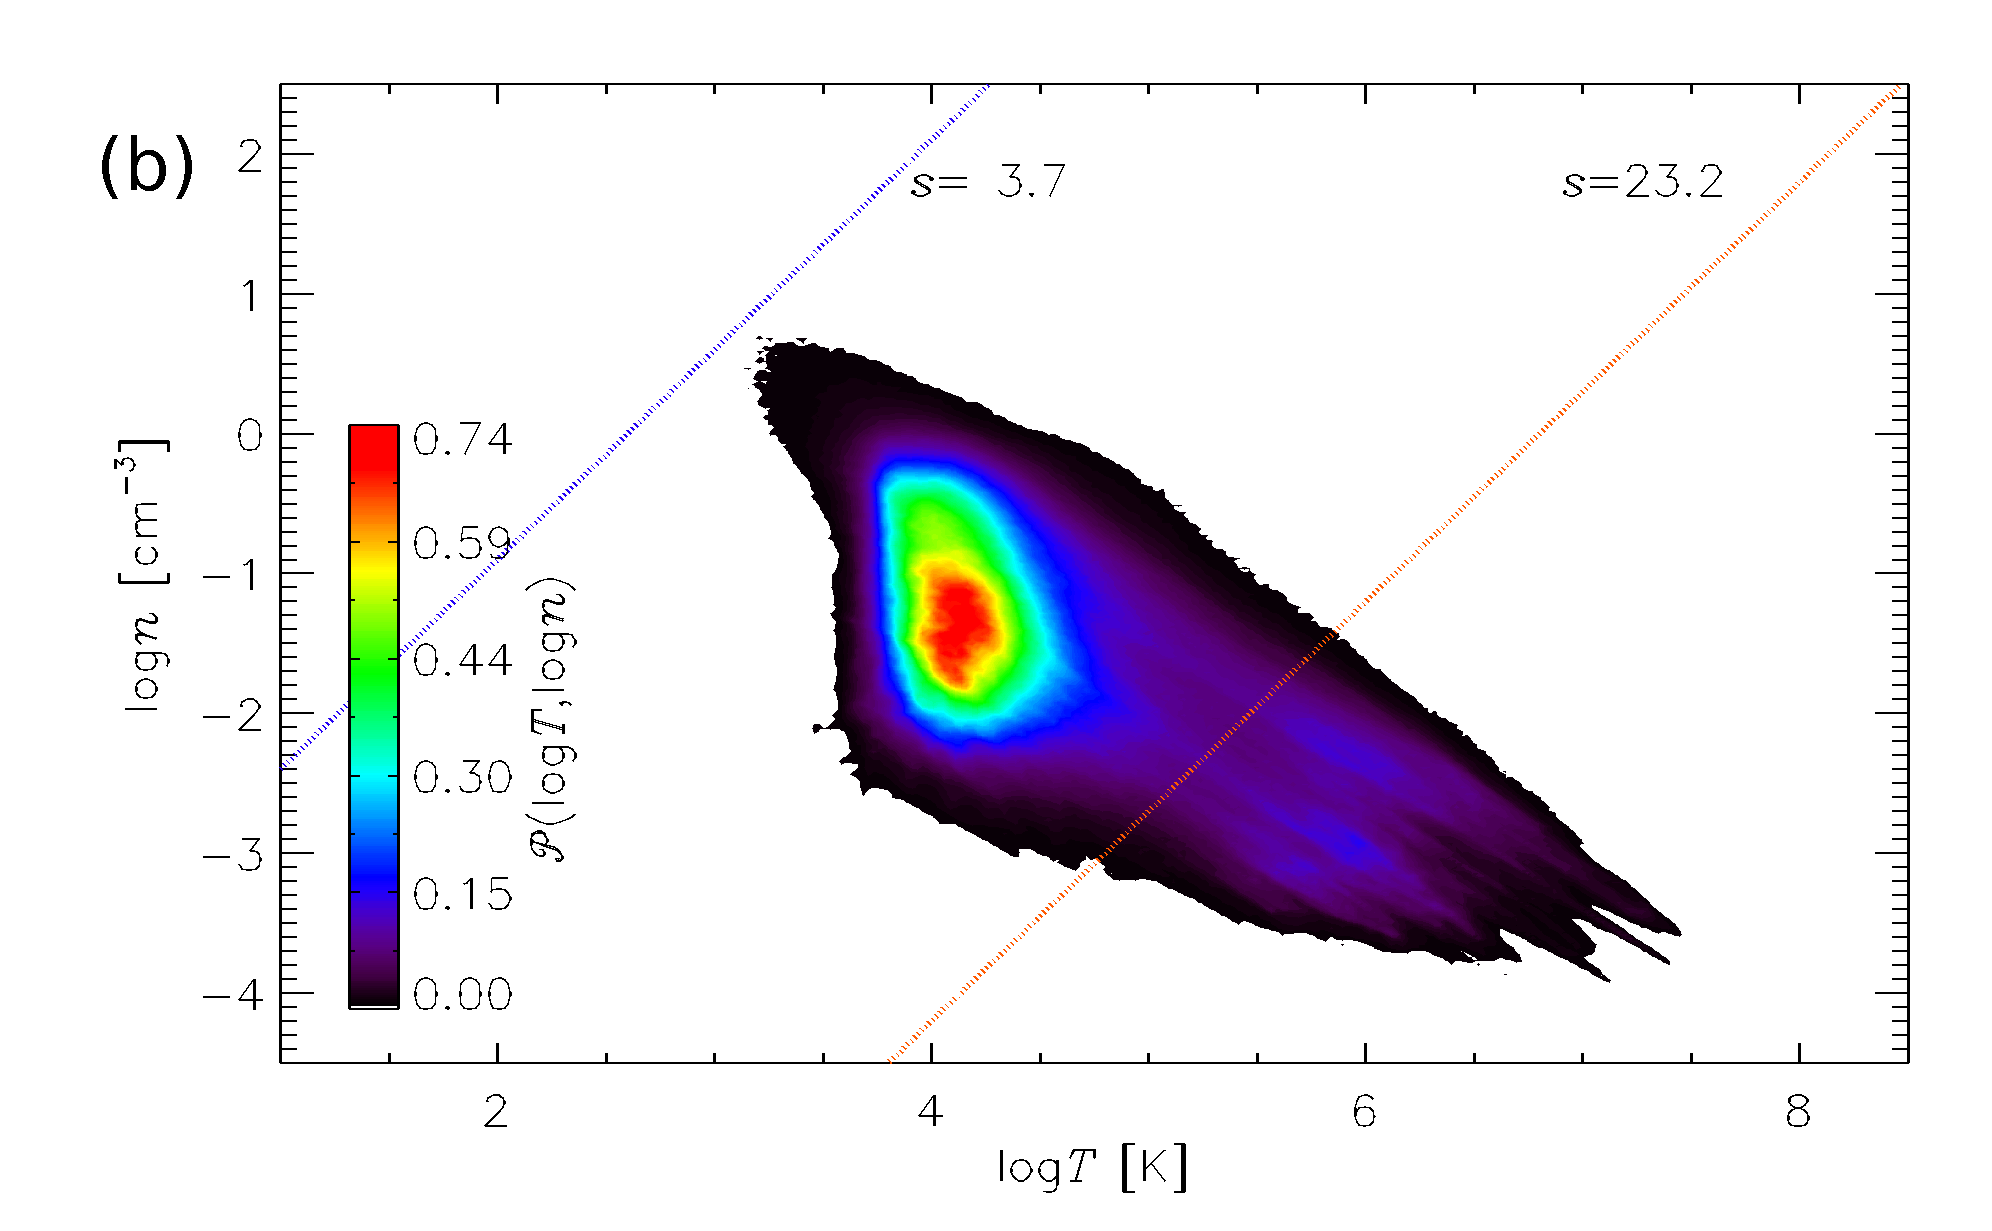
\includegraphics[width=0.9\linewidth]{fig/o1ph_pdf2dtn.png}
    \caption[2D probability distribution of $n$ and $T$ for Models~$\Ompa$ and $\Omph$]{
  Probability contour plot by volume of log$n$ vs log$T$ for Model~$\Ompa$
  {\textbf{(a)}}
  and Model~$\Omph$ {\textbf{(b)}}.
  The lines of constant entropy $s=4.4\cdot10^{8}$ 
  and $23.2\cdot10^{8}\erg\g^{-1}\K^{-1}$ indicate where the phases are defined
  as cold for $s\le4.4$ and as hot for $s>23.2$. 
  \label{fig:b2dv}
    }
  \end{figure}
%-----------------------------------------------------------------------------

  Comparing the combined probability distribution of density and temperature
  for both of these models in Fig.~\ref{fig:b2dv} with those of Model~\Op\
  in \cite[][Fig. 5.10]{Gent12} the spread is more broad and not obviously 
  aligned along a line of constant pressure.
  The HD distribution here is less compact than with MHD. 
  However when considering only the mid-plane distributions, as displayed in
  Fig.~\ref{fig:b2dh} the distributions match better with Model~\Op\ and the 
  pressure alignment is evident.
  So the broad distributions for the total volumes are explained by the 
  stronger gradient in the pressure distribution, due to the reduced 
  stirring of the hot gas.
  The thermal pressure at the mid-plane is also very similar in both models,
  reflected also in the agreement of the total and thermal pressure near the
  mid-plane in the plot of horizontal averages (Fig~\ref{fig:zrhom}b).
  The magnetic and turbulent pressure in Model~$\Ompa$ combine to match the
  mid-plane turbulent pressure alone of Model~$\Omph$.
  For the temperature in Model~$\Ompa$ the hot gas has two modes, evident in 
  Fig.~\ref{fig:b2dv}a at $10^5\K$ and $10^6\K$, but at the mid-plane there 
  only the single $10^3\K$ mode. 
  The structure of the ISM at the mid-plane is therefore common to both models
  with modes at $10^6\K,~10^{-2}\cmcube$ and $10^4\K,~1\cmcube$.
  The cold gas is insufficiently resolved in Model~$\Ompa$ for comparison. 
  
%-----------------------------------------------------------------------------
  \begin{figure}
  \centering
  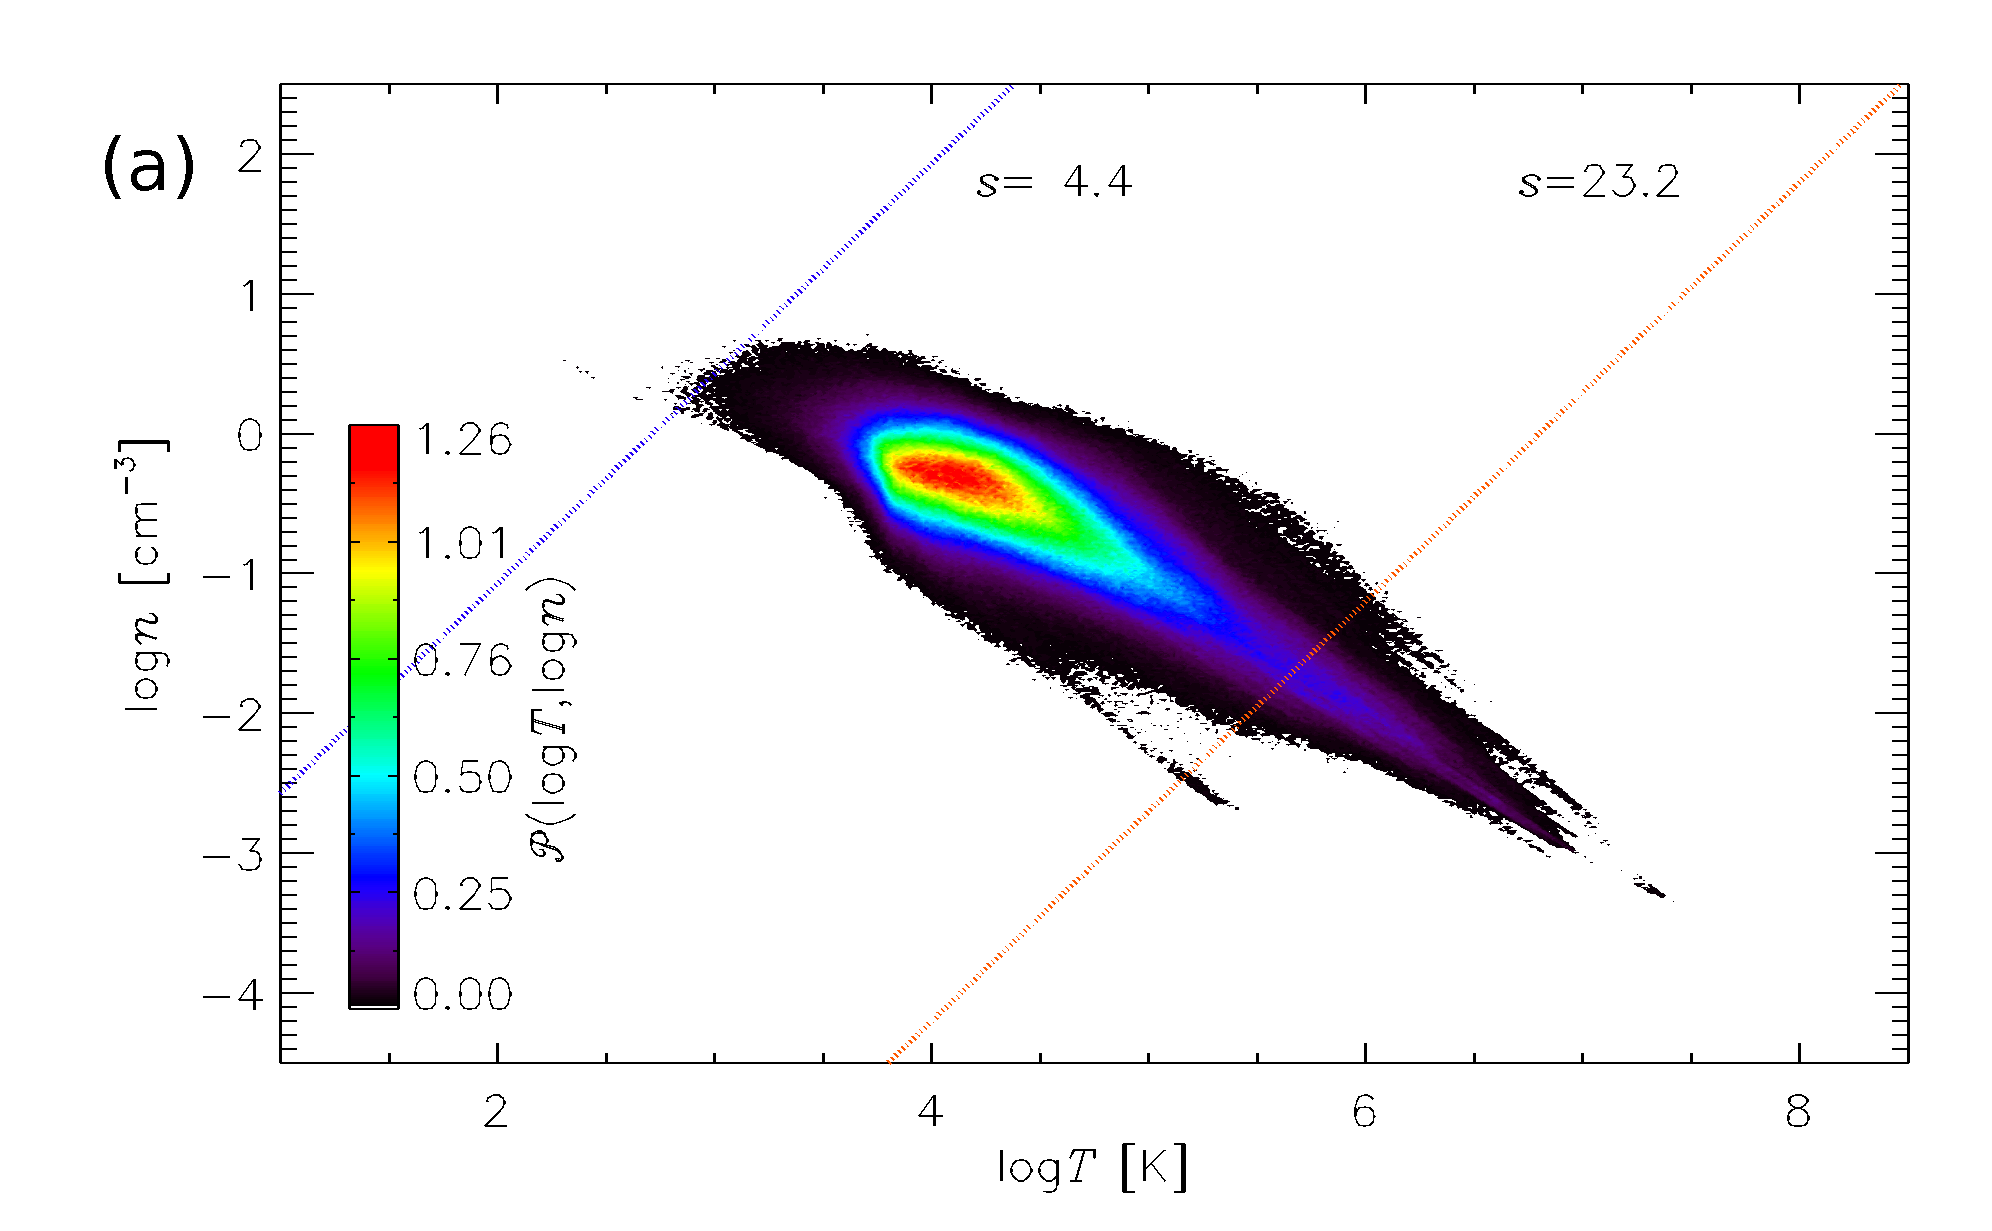
\includegraphics[width=0.9\linewidth]{fig/o1pr_pdf2dh.png}  
  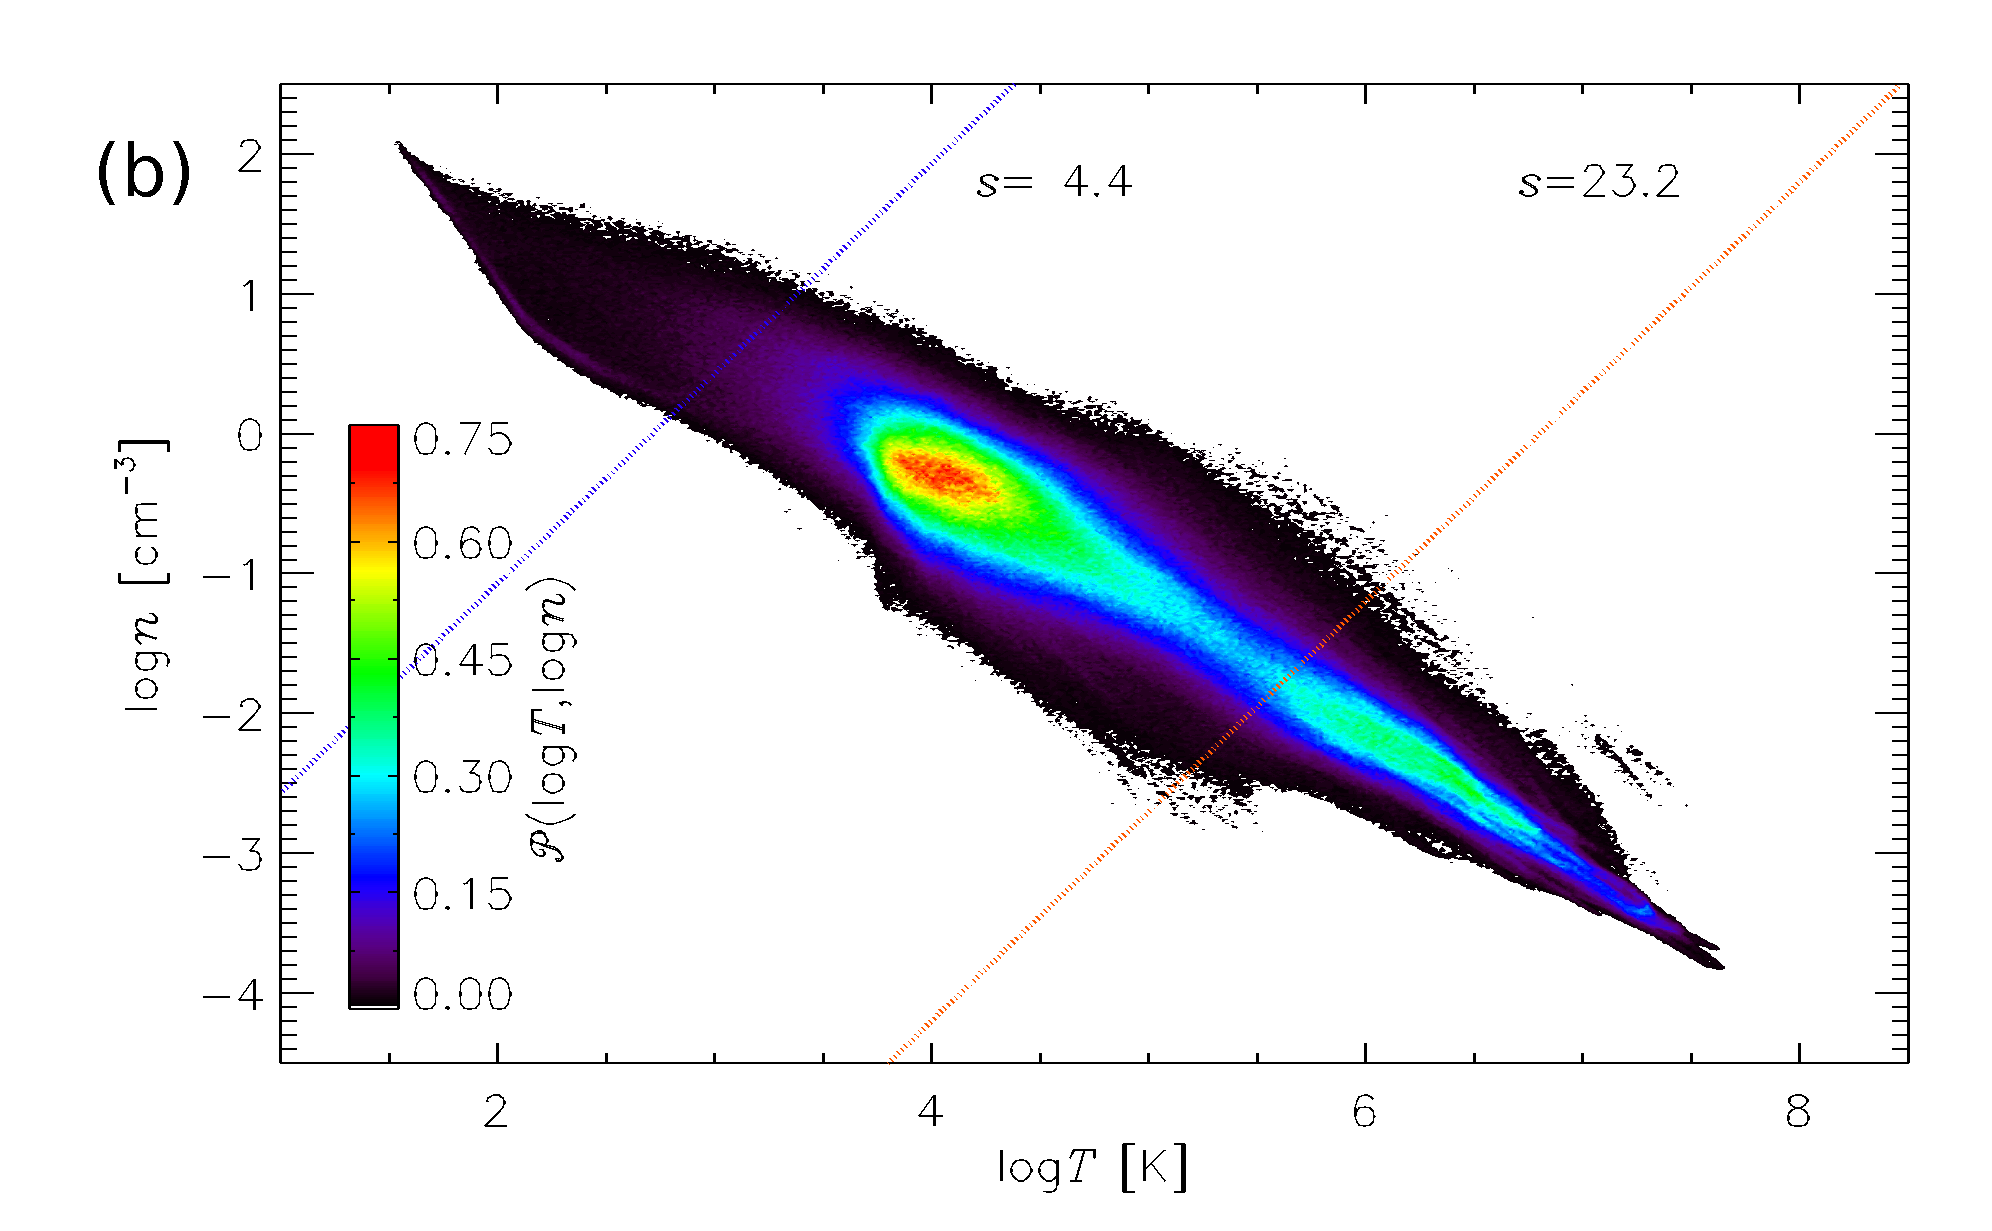
\includegraphics[width=0.9\linewidth]{fig/o1ph_pdf2dh.png}
    \caption[2D mid-plane probability distribution for Models~$\Ompa$ and  $\Omph$]{
  The mid-plane probability distributions ($|z|<100\pc$) by gas number density 
  $\log n$ and temperature $\log T$ for {\textbf{(a)}} Model~$\Ompa$ and
  {\textbf{(b)}} Model~$\Omph$.
  \label{fig:b2dh}
    }
  \end{figure}
%-----------------------------------------------------------------------------

  There is no evident dependence in the probability distributions between the 
  MHD models differing in rotation, shear or SN rate.
  The models in the kinematic stage extend to lower densities and higher 
  temperatures than either the HD Model~$\Omph$ or the MHD models in the 
  dynamo saturated state, and also extend to lower pressures.
  
%-----------------------------------------------------------------------------
  \begin{figure}
  \centering
  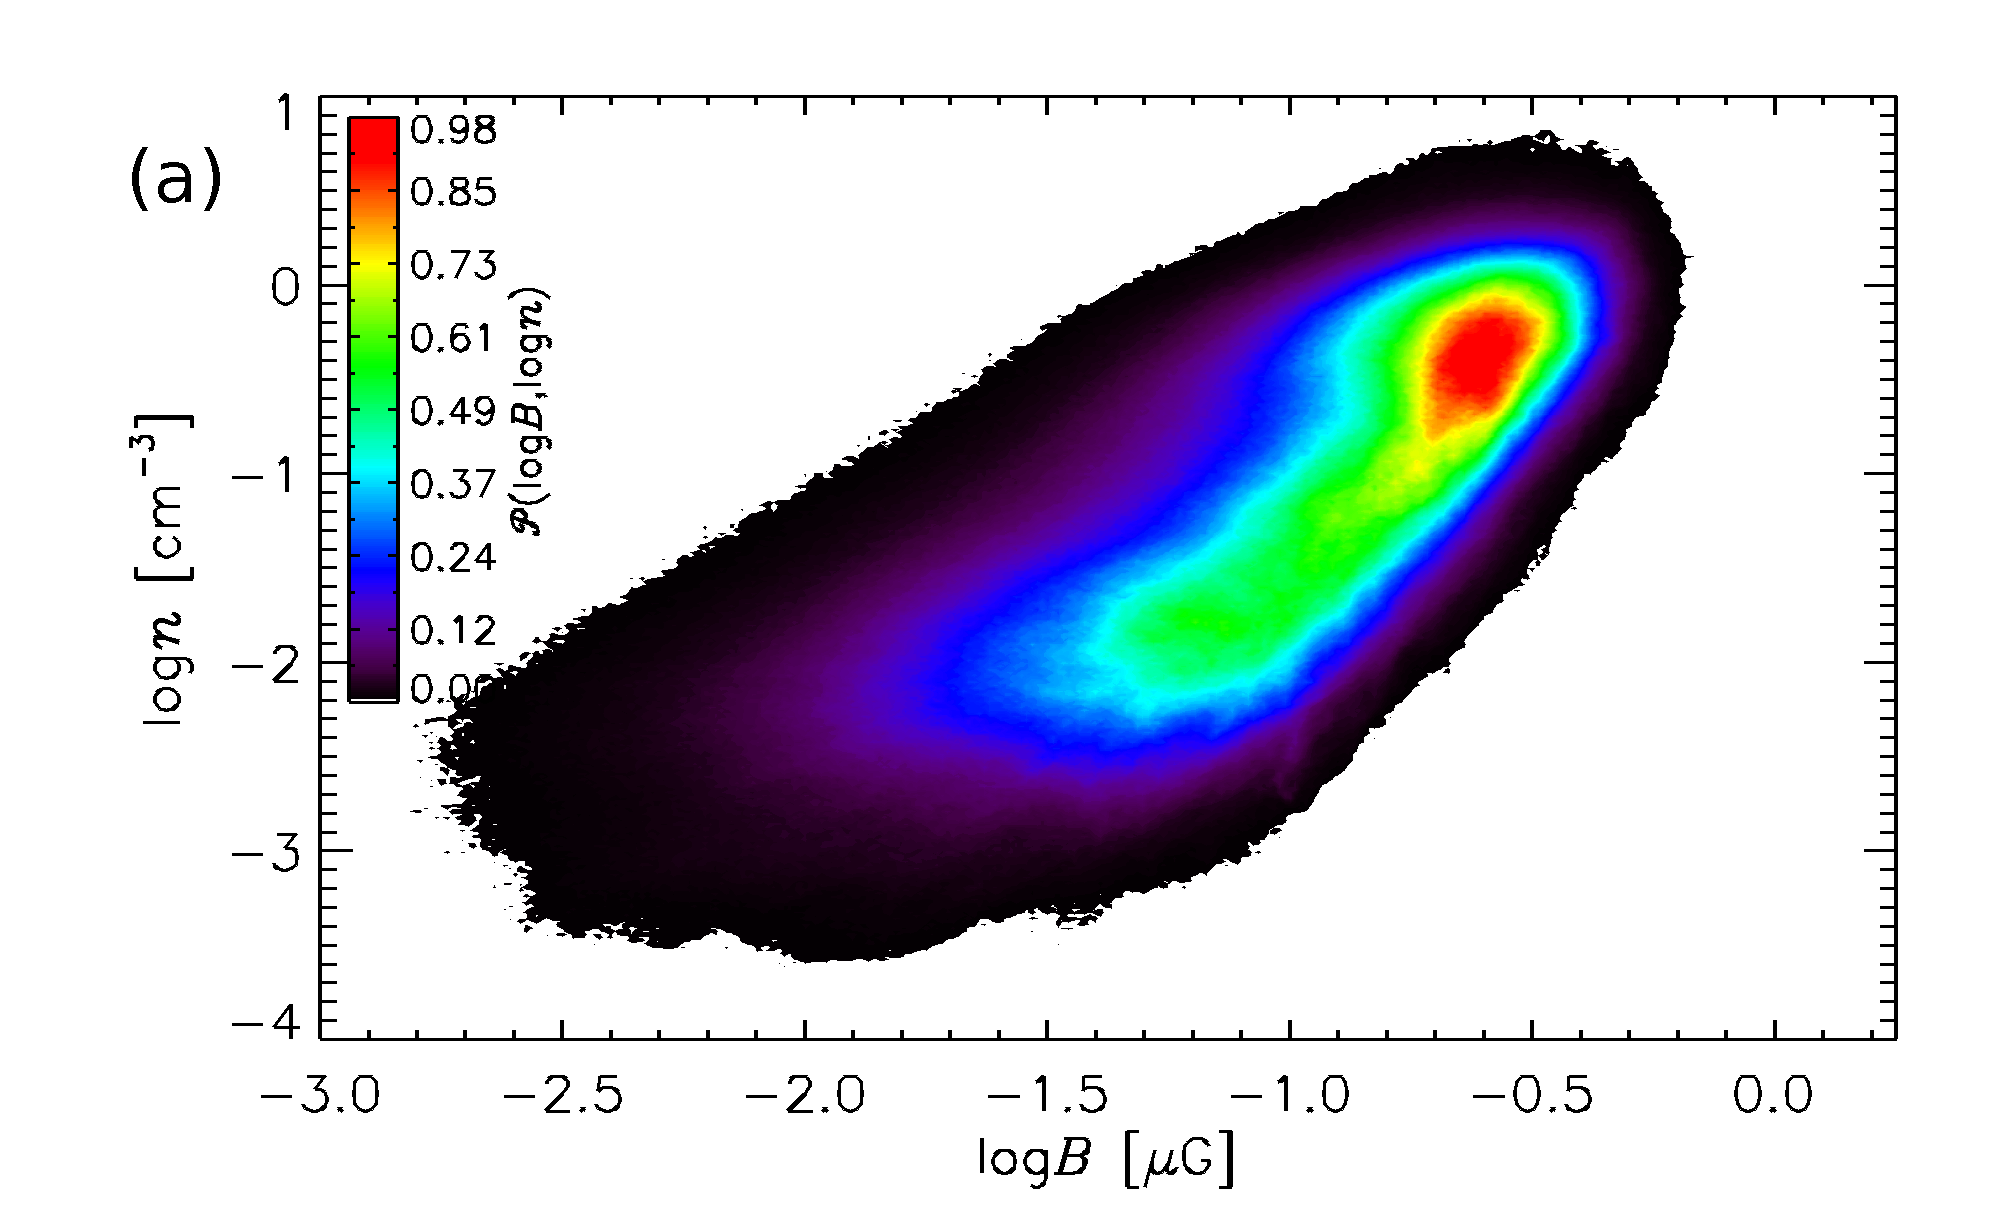
\includegraphics[width=0.9\linewidth]{fig/o1pr_pdf2db.png}  
  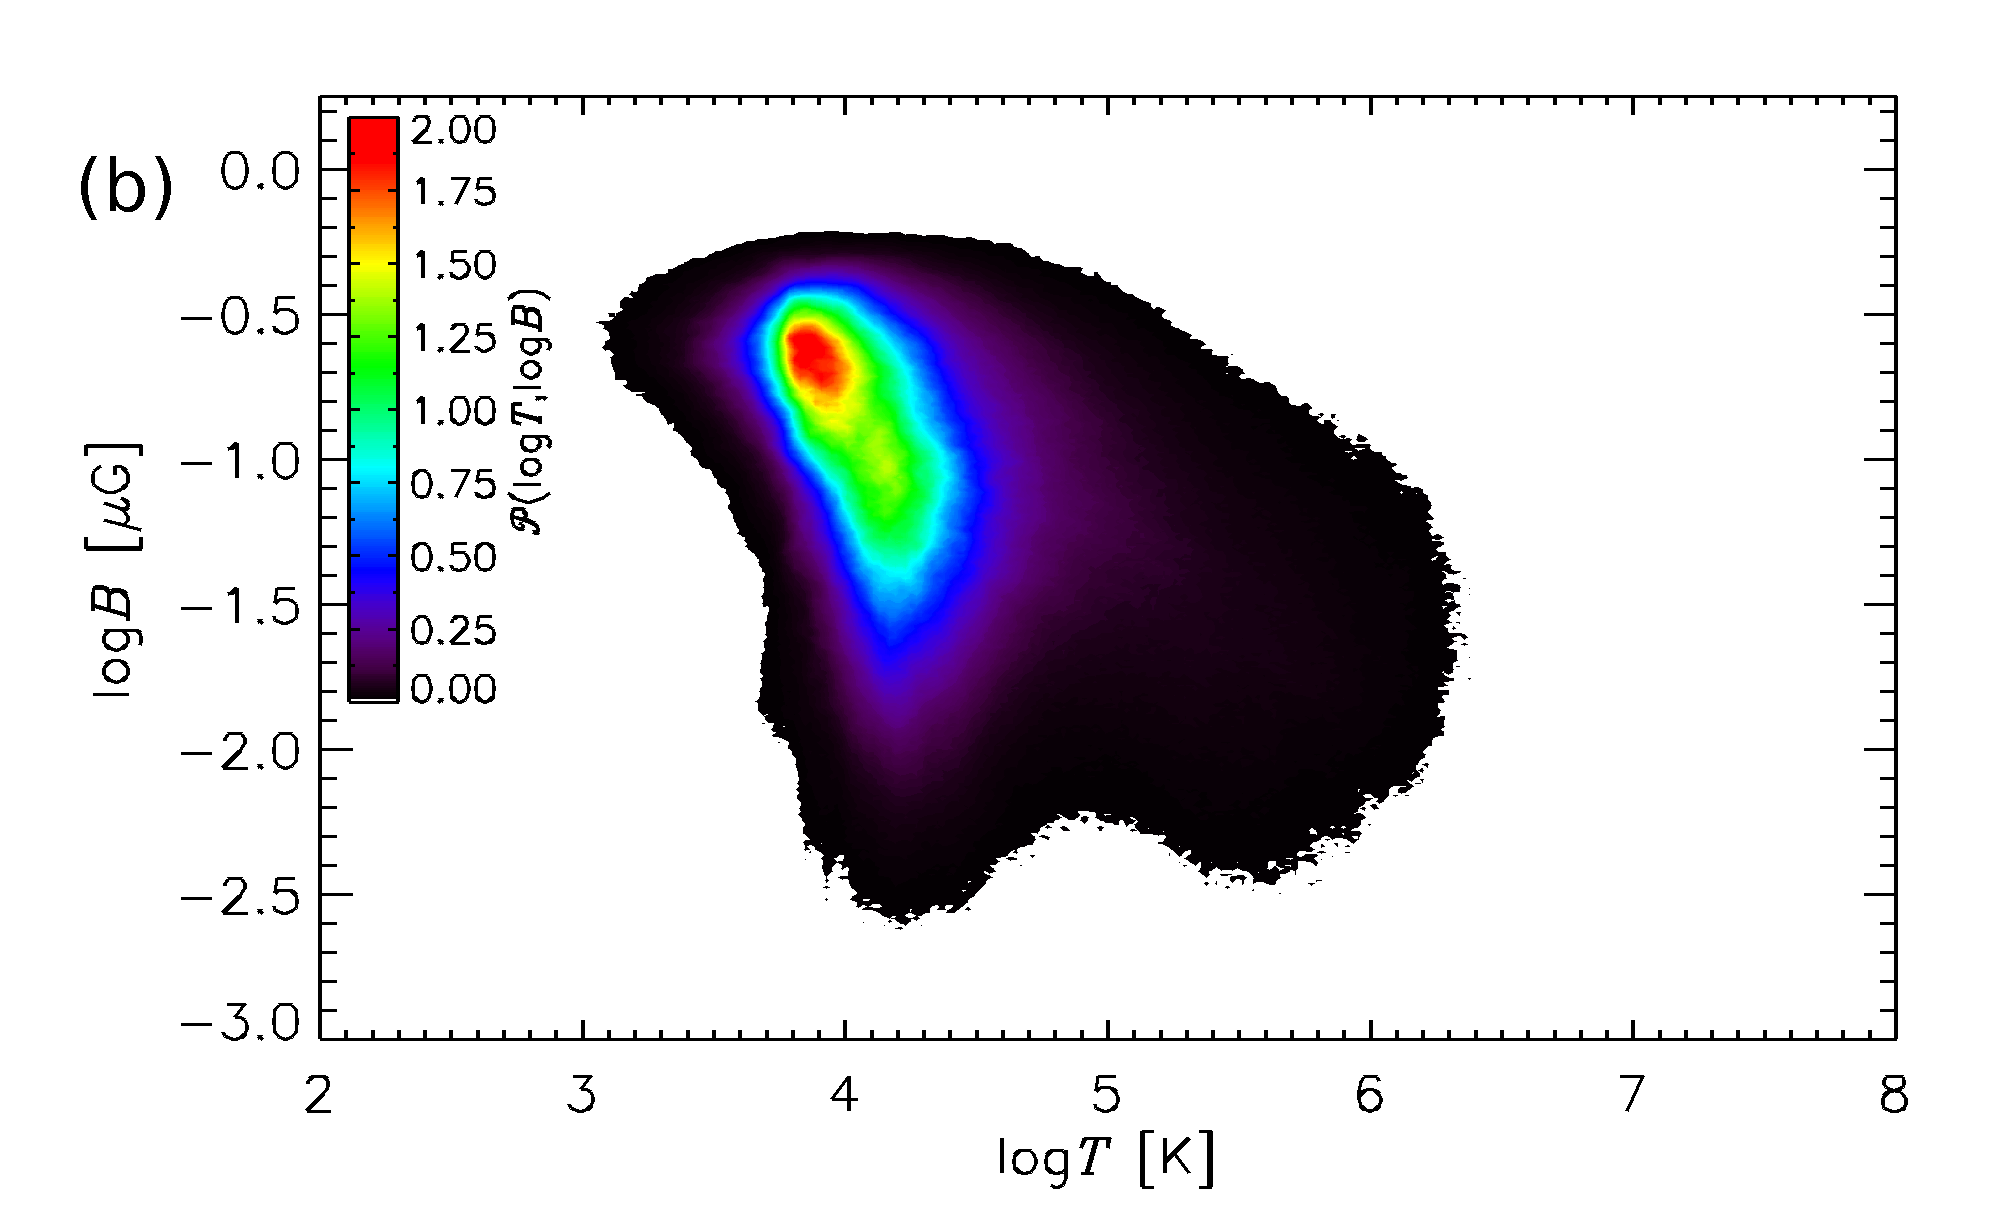
\includegraphics[width=0.9\linewidth]{fig/o1pr_pdf2tb.png}
    \caption[2D probability distribution of $n,B$ and $B,T$ for Model~$\Ompa$]{
  Total volume probability distributions ($|z|<100\pc$) by gas number density 
  $\log n$ and magnetic field strength $\log |B|$ {\textbf{(a)}} and
  temperature $\log |T|$ and magnetic field strength $\log |B|$ 
  {\textbf{(b)}} for Model~$\Ompa$.
  \label{fig:b2dnt}
    }
  \end{figure}
%-----------------------------------------------------------------------------

  In Fig.~\ref{fig:b2dnt}a the joint probability distributions of gas number 
  density with magnetic field strength is shown and in Fig.~\ref{fig:b2dnt}b
  of temperature with magnetic field strength for Model~$\Ompa$.
  From (a) it is clear there is a strong positive correlation between magnetic
  field strength and density and from (b) a weak negative correlation between
  temperature and field strength.
  The $T,B$ distribution has very strong peak at $T=10^4\K$.  
  
  
%-----------------------------------------------------------------------------
  \begin{figure*}
  \centering
  \hspace{-1.25cm}
  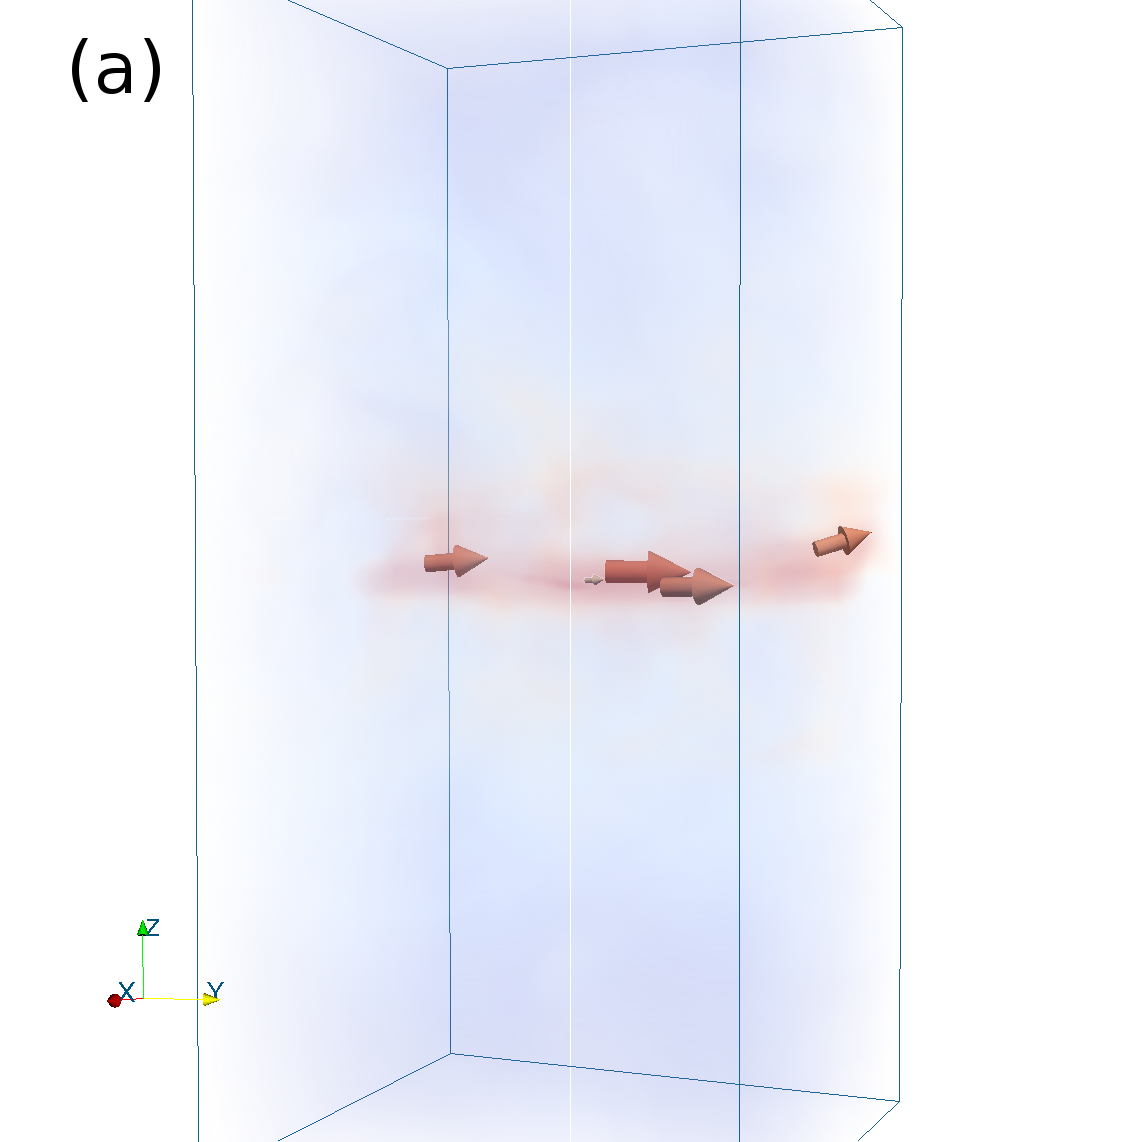
\includegraphics[width=0.35\linewidth]{fig/b310c.png}\hspace{-1.15cm}
  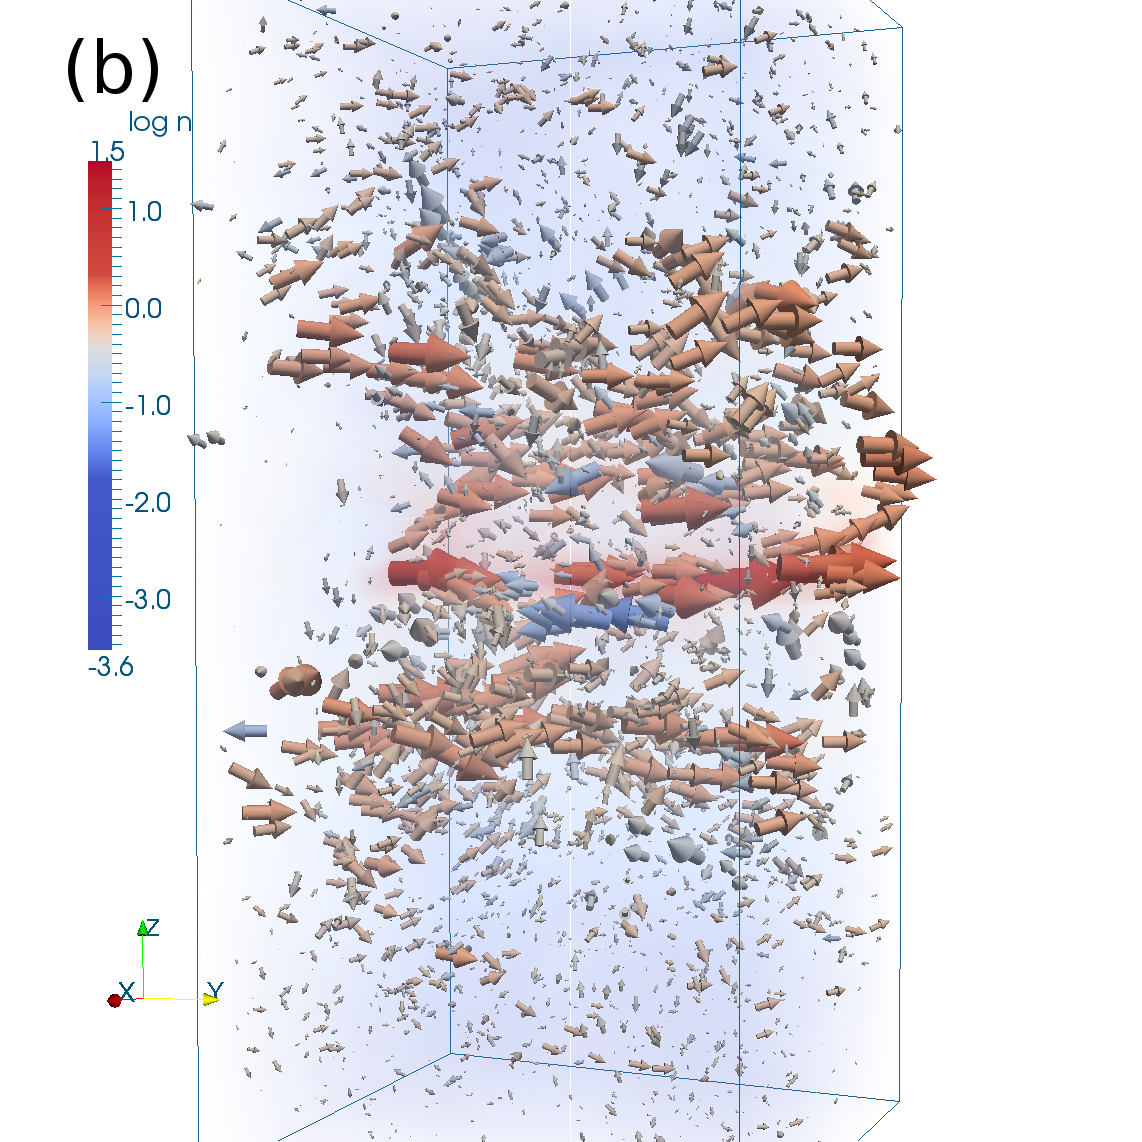
\includegraphics[width=0.35\linewidth]{fig/b310w.png}\hspace{-1.15cm}
  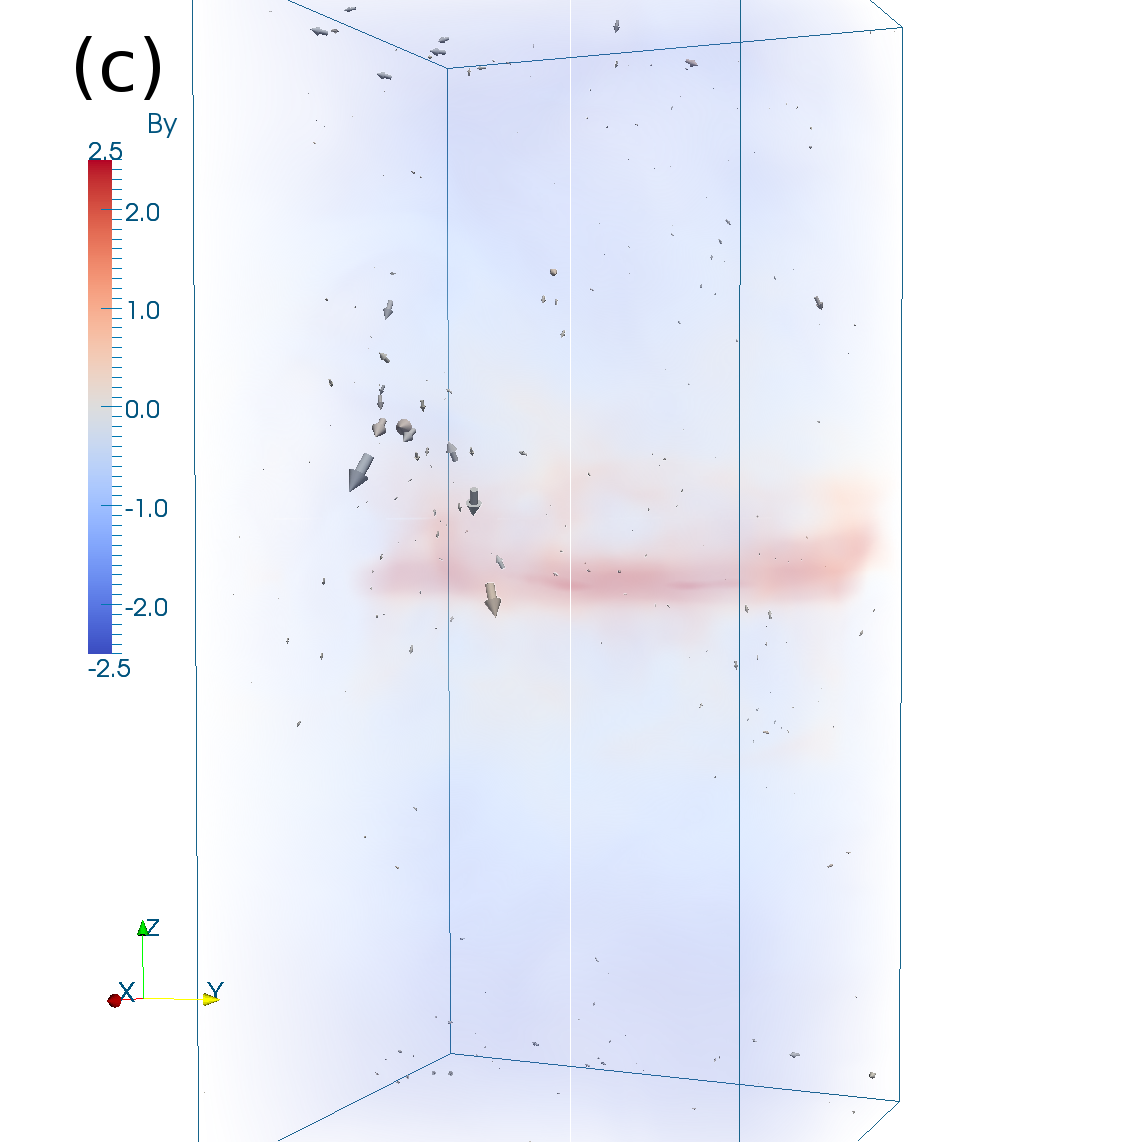
\includegraphics[width=0.35\linewidth]{fig/b310h.png}
  \hspace{-1.25cm}
  \caption[Volume snapshots of $\vect{B}$ by phase for Model~$\Ompa$]{
  Vector plots of the magnetic field $\vect{B}$ {\text{(a)}} in the cold phase
  {\text{(b)}} the warm phase and {\text{(c)}} the hot phase.
  Field directions are indicated by arrows and strength by their thickness.
  The colour of the arrows indicates the strength of the
  azimuthal ($y$) component (colour bar on the right).
  The background shading illustrates the density of the ISM.
  \label{fig:b3box}}
  \end{figure*}
%-----------------------------------------------------------------------------

  For Model~$\Ompa$ the ISM for a single snapshot is decomposed into the 
  three phases and the magnetic field for each plotted separately in 
  Fig.~\ref{fig:b3box}.
  In panel a the cold gas occupies only a limited volume near the mid-plane, 
  but the magnetic field is very strong and organised in alignment with the
  mean field surrounding it in the warm gas. 
  This is represented by the length and thickness of the vector arrows.  
  The colour of the arrows emphasises that the alignment has a strong 
  azimuthal component. 
  No arrows are present away from the mid-plane, because the cold gas is absent 
  there.
  In panel b the warm gas is present throughout the numerical volume.
  Field vectors are present almost throughout and the field is highly aligned,
  mainly in the azimuthal direction. 
  The strength of the field increases towards the mid-plane.
  The presence of some vectors in blue or grey indicates that there are 
  significant perturbations where the field includes reversals, some of these
  strong.
  Some of the field exhibits significant vertical orientation, but it is 
  mainly horizontal.
  In panel (c) the hot gas is also present throughout the volume, although 
  in smaller amounts near the mid-plane. 
  Despite this there is very little magnetic field.
  What field there is generally weak and lacks much systematic alignment, 
  although any orientation tends to be vertical, consistent with the
  field lines being stretched by the gas flowing away from the mid-plane. 
  Effectively the hot gas has a very weak field, which is highly disordered.
  Most of the magnetic field, and particularly the mean field, occupies the 
  warm gas.
  Detailed quantitative analysis of the structure of the gas will be deferred to
  future work.


  \section{Summary}
  The magnitude of the magnetic field is strongly aligned to the density of the
  ISM and indirectly the warm and cold phases.
  More particularly the mean field is stronger in the warm and cold gas, with 
  the hot gas containing a more random field. 
  The mean magnetic field and the magnetic energy is strongest at 
  $|z|\simeq300\pc$, just outside the SNe active region. 
  The fluctuating dynamo is likely to be strongest in this SNe active region,
  but due to the low magnetic Reynolds numbers in the simulations, it is likely
  that the field and energy is significantly weaker in the simulations than 
  might be expected.





%end FAG
\section[]{Field lines of the magnetic field}
Field lines of the magnetic field give a qualitative description of the magnetic field in the ISM. We introduce sampling of physical variables along the field lines of the magnetic field, to obtain a quantitative description of the observables. Observables, such as entropy or pulsar RM measures \citep{SSFS02} are frequently used to derive other observables or statistics.  The use of sampling along field lines will enable the analysis of observables across many snapshots, whilst avoiding the use of time averages, which is not sensible for observables associated to a turbulent flow \citep{TL72}. For example, the wavelet transform methods used by Stepanov \textsl{et al} \citep{st02} are used to derive the Galactic magnetic field from pulsar RM data. Field lines of the Galactic magnetic field can be derived from this analysis and it can be further analysed using sampling along the field lines.\\
The mean magnetic field is considered first, to explore the large-scale characteristics of the magnetic field, having extracted the random, small-scale fluctuations with Gaussian volume averaging.  Intuition suggests that the mean magnetic field will prefer to stay in the warm phase, which provides a less hostile environment for the magnetic field than the transonic, compressible turbulence of the hot phase. This will be discussed using the field lines and by comparison with a test case.
\boldmath
\subsection{Field line equation for a vector field, $\bvec{A}(\bvec{x})$}
\unboldmath
Given a vector field, $\bvec{A}(\bvec{x})$, in Cartesian coordinates, its field lines are described by
\begin{equation}
\frac{dx}{A_{x}}=\frac{dy}{A_{y}}=\frac{dz}{A_{z}}=ds,
\label{f_lines_eqn}
\end{equation}
where $ds$ is a separation constant used to integrate along the field line. This is formulated as
\begin{equation}
\begin{cases}
\frac{dx}{ds}=A_x,\\
\frac{dy}{ds}=A_y,\\
\frac{dz}{ds}=A_z,
\end{cases}
\label{fld_eqns}
\end{equation}
 The field line equation is integrated along $x$, $y$ and $z$ to obtain the field lines,
\[L: (x(s),y(s),z(s)),\]
which are integrated using a $4^{th}$-order Runge-Kutta scheme. For discrete-valued $\bvec{A}(\bvec{x})$ interpolation is used to evaluate its components at positions, $\bvec{x}$, which do not lie on the data grid. 
\subsection{3D rendering of field lines of the mean magnetic field}
\begin{figure*}
  \vspace{0cm}
  \centering
\hspace*{0cm} 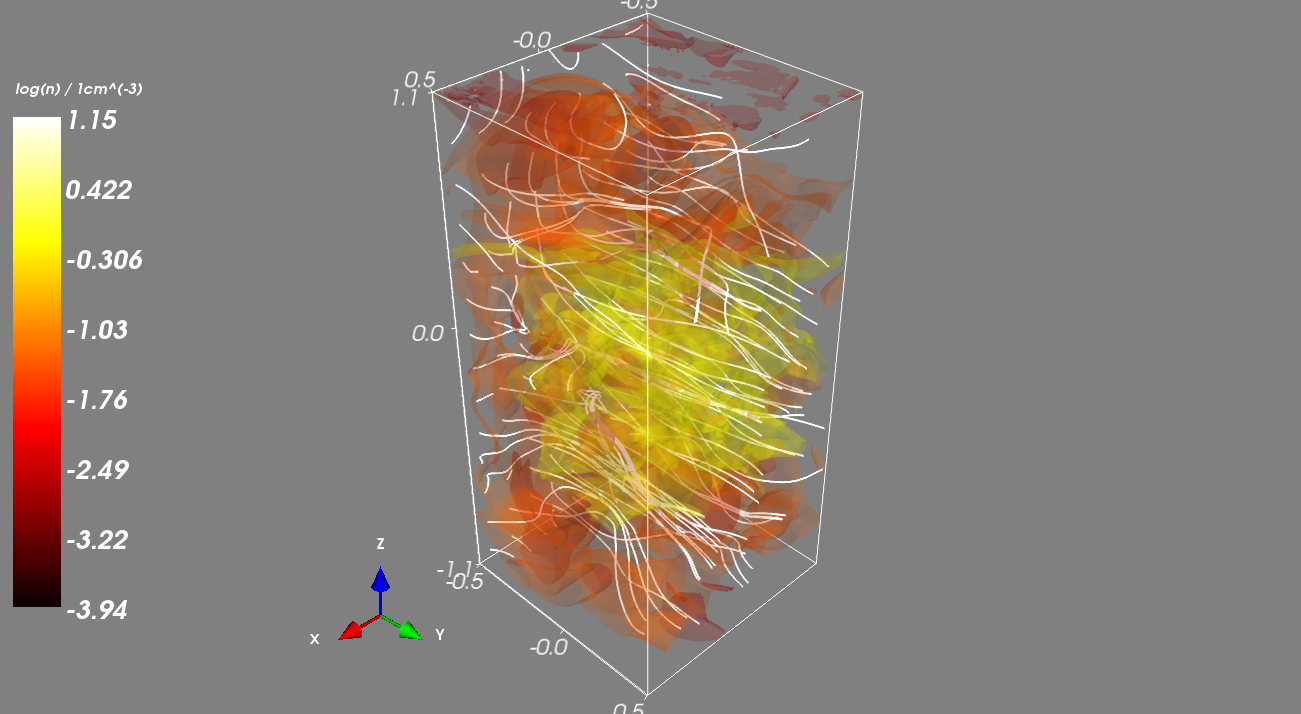
\includegraphics[width=\linewidth]{snapshot1.png}
\hspace*{0cm} \caption{3D rendering of the field lines of the mean magnetic field. The white lines are field lines seeded along a regular grid on the $xz$-plane at $y\approx-0.5$ kpc. 
  \label{fig:fld_lines}}
  \end{figure*}
\begin{figure}
\centering
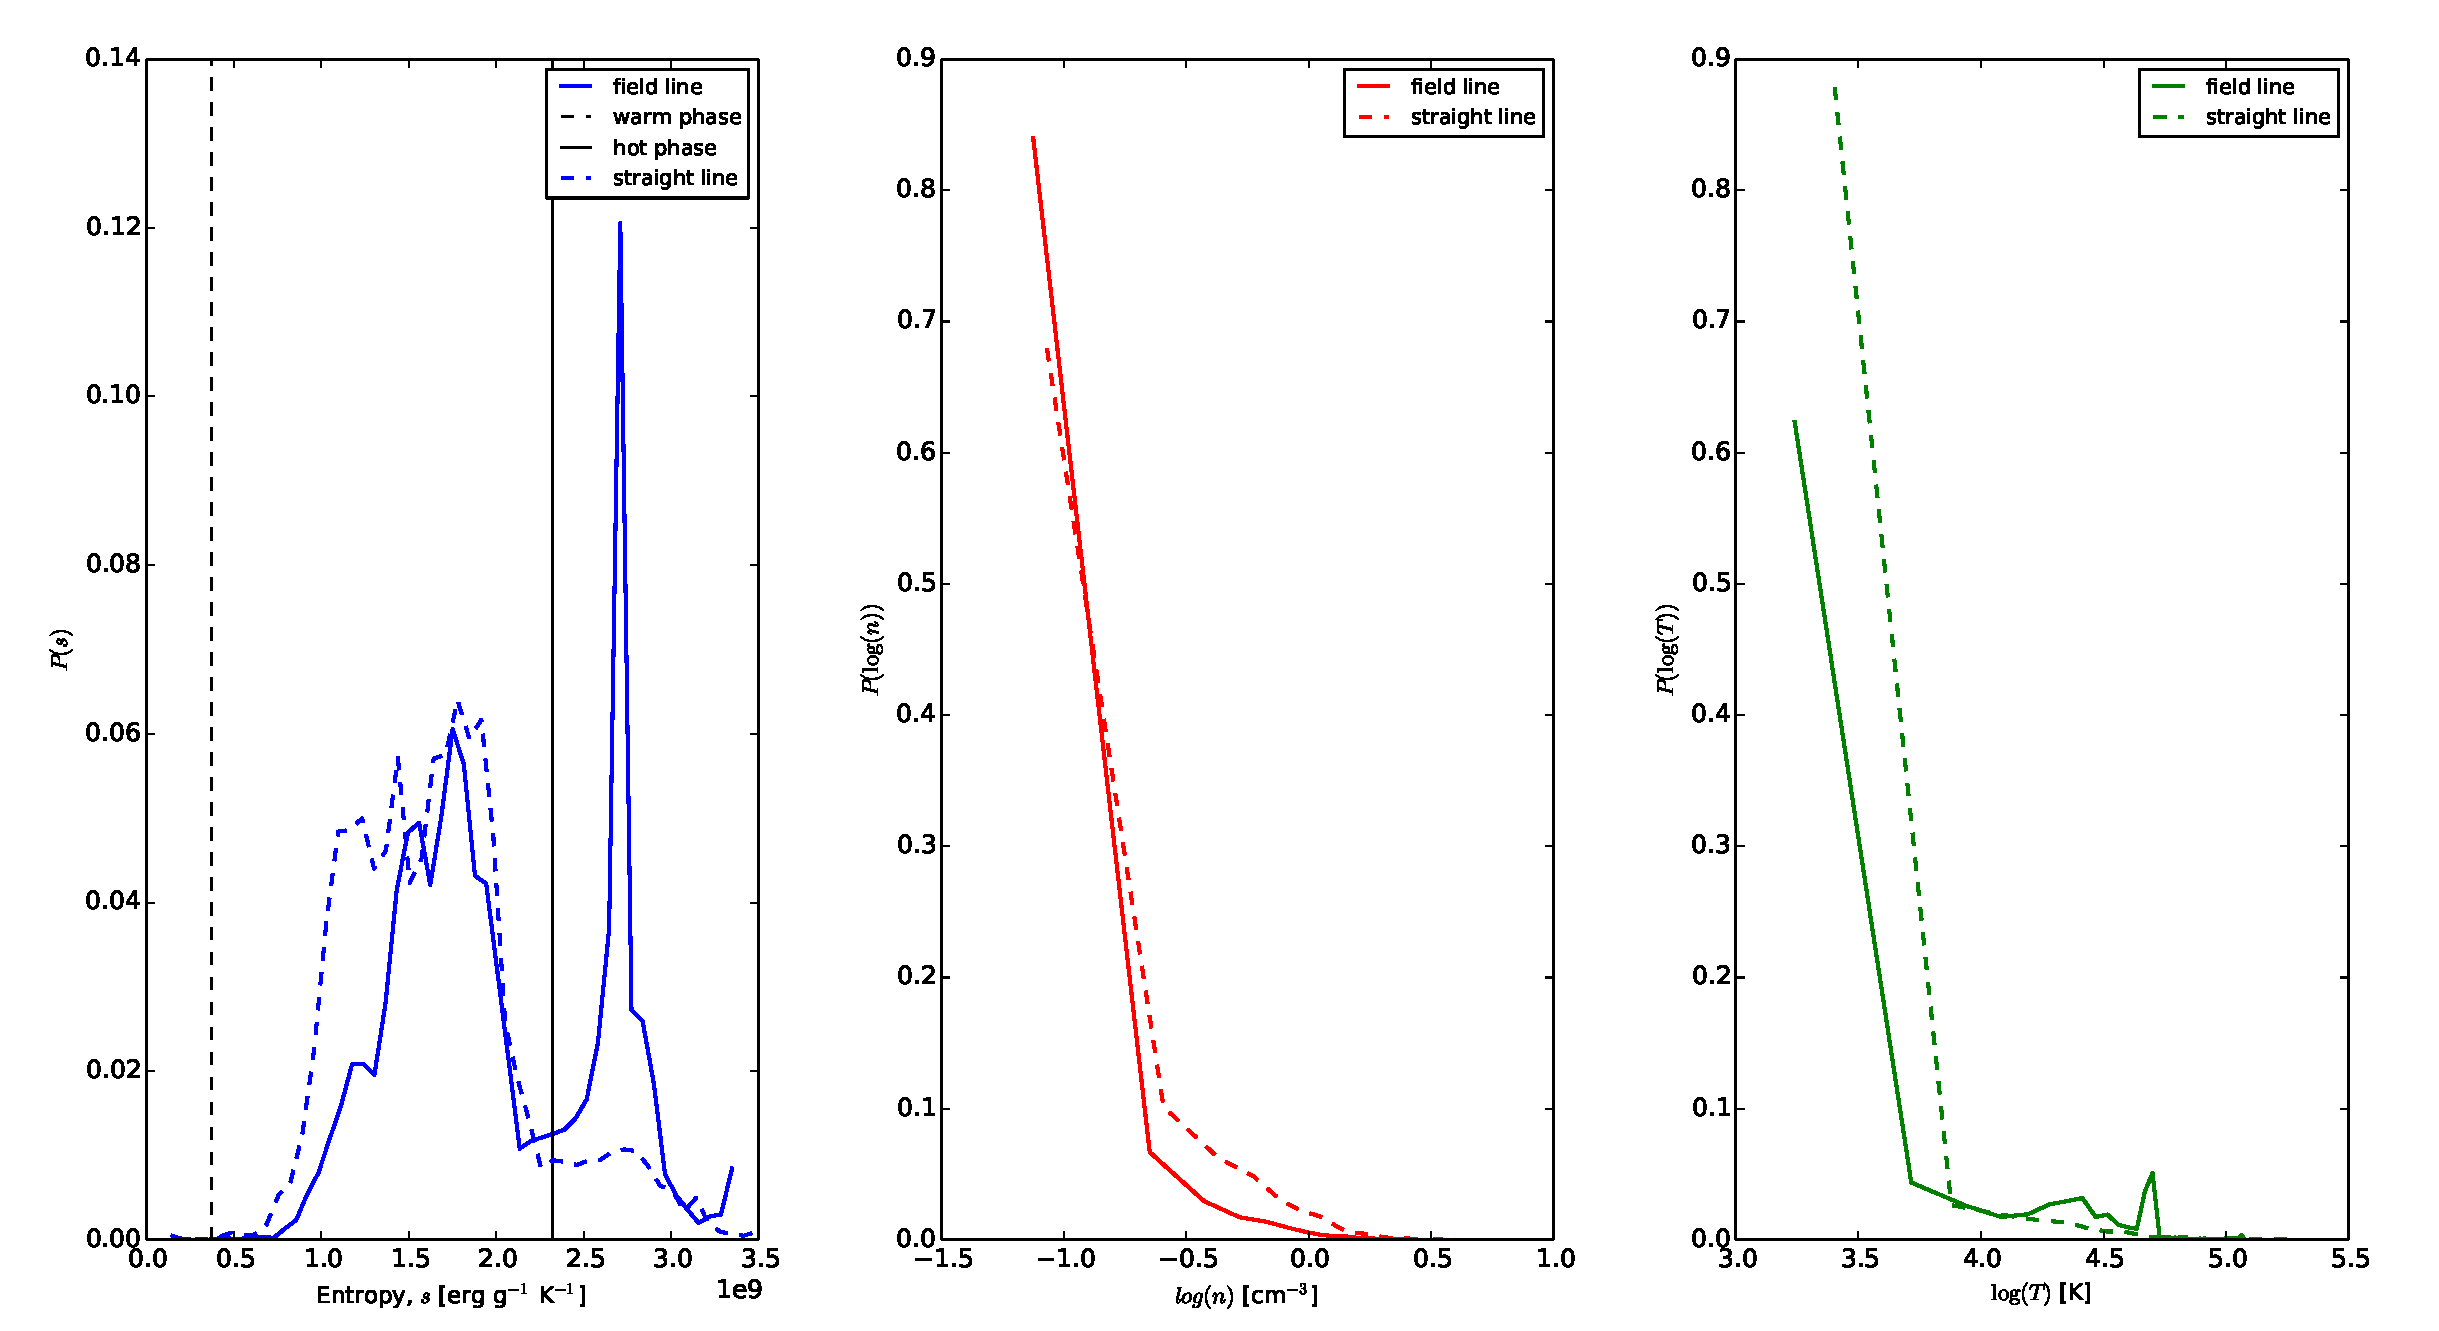
\includegraphics[width=\linewidth]{sline_vs_fld1.pdf}
\caption{PDFs of entropy (blue), $s$, log density (red), $\log(n)$, and log temperature (green), $\log(T)$, along field lines (solid) and straight lines (dashed).}
\label{fig:pdfs_mean}
\end{figure}
In Figure \vref{fig:fld_lines}, the white field lines have been seeded along the $xz$-axis at $y\approx-0.51$ kpc. The translucent gas inside the box is a representation of the log density, $\log(n)$, field. Density decreases from brighter to darker colours. Since the warm and hot phase represents approximately $\%99$ of the fractional volume of the ISM gas, it is only useful for visualising the characteristics of the field line within the warm and hot phases. We will present a preliminary result regarding the field lines within the cold phase in this paper. However, a more detailed discussion will be reported elsewhere. 
For descriptive purposes, the yellow shades of gas correspond to warm gas and the red shades correspond to the hot phase. We note that the field lines are generally aligned with the positive $y$-direction, especially in the warm phase and the field lines are smooth inside the warm gas. However, we notice significant differences in the characteristics of the field lines in the hot phase.\\ 
There is an isolated structure of hot gas (likely to be a SN remnant) in the (approximate) range $-0.8<z<-1.1$ kpc. The field lines in this region still traverse the computational domain in the positive $y$-direction. However, they are distorted and stretched in the positive $z$-direction in the region surrounding the hot gas.\\  
Similarly, in the range $0.7<z<1.1$ kpc, there is a larger structure of hot gas, which spans the $xy$-plane. This structure appears to be part of rising hot gas, which is leaving the computational domain. As it leaves, it elongates the magnetic field lines until they are no longer connected inside the domain. Consequently, the the field lines are approximately perpendicular to the $y$-axis, where the stretching of the field lines occur due to the hot phase. (NEED TO CHECK WHETHER THE MAGNETIC FIELD ENERGY IS STRONGER IN THESE REGIONS COMPARED WITH THE STRAIGHT LINES!)
\subsection{A Test: Comparison of probability density functions (PDFs) along field lines with PDFs along straight lines}
Even though the visualisation is informative, it is necessary to determine whether the field lines are sensitive to the phases of the ISM. Consequently, we compare the characteristics of the field lines against straight lines launched in the positive $y$-direction, from the seed points used to compute the field lines. This test is devised using ideas from the field of stereology \citep{BJ04}, lineal analysis in particular. The straight lines used in the test case will have the same general characteristics as the field lines, since they both traverse the computational domain in the positive $y$-direction. This ensures that the lines are representative of the field lines being sampled. Despite having the same general characteristics, the straight lines should not be sensitive to the phases of the ISM; they will not prefer to stay in a particular phase, whilst avoiding others. Therefore, comparison of the PDFs of the observables sampled along the field lines and the straight lines, should identify sensitivity (or lack thereof) of the field lines to the phases of the ISM.\\
\noindent Figure \vref{fig:pdfs_mean} shows the probability density functions (PDFs) of entropy, log density and log temperature sampled along field lines (solid lines) and straight lines (dashed lines). The PDFs for log density and log temperature suggest that the PDFs have similar overall behaviour, which is most likely due to their alignment in the $y$-direction. This is reassuring since the choice of aligning the straight lines in the $y$-direction was to avoid introducing uncharacteristic behaviour into the comparison. The straight lines have the orientation of the field lines, without the sensitivity to phases.\\
We now consider the PDFs entropy along the field lines and straight lines in Figure \ref{fig:pdfs_mean}. These PDFs are more rich in information. Firstly, we observe similar peaks in the region $1.66<s<10.365$, which corresponds to the warm phase. This agrees with Figure \vref{fig:fld_lines} in that the field lines do not seem sensitive to the warm phase. \\
\begin{table}[H]
 \centering
 %\begin{minipage}{180mm}
  \caption{Respective probabilities of finding the field and straight in the cold, warm and hot phases.}
  \label{table:mean_probs}
 % \begin{tabular*}{@{}c c c @{}}{\linewidth}{@{\extracolsep{\fill}}p{0.3\linewidth}p{0.3\linewidth}p{0.3\linewidth}@{}}
\begin{tabular*}{\linewidth}{@{\extracolsep{\fill}}p{0.3\linewidth}p{0.3\linewidth}p{0.3\linewidth}@{}}
  \hline
   Probability& Field lines& Straight lines \\
 \hline
\\
$\mathcal P(\text{cold phase})$&$8.384\cdot10^{-5}$ &$7.818\cdot10^{-4}$  \\
   $\mathcal P(\text{warm phase})$& $0.6577$&$0.8865$   \\
   $\mathcal P(\text{hot phase})$&$0.3422$ & $0.1127$    \\
\hline
\end{tabular*}
%\end{minipage}
\end{table}
\noindent We observe a sharp peak for the PDF of entropy along the field line, centred at $s\approx27\cdot10^8$ erg g$^{-1}$ K$^{-1}$, which is inside the hot phase. A similar peak is not observed for the PDF of entropy along the straight line. This can be explained by the field lines being stretched by the hot gas and thus traversing the hot phase for a higher proportion of their length than the straight lines, which are not affected by stretching. We formulate probabilities of traversing each phase for the field lines and straight lines from their PDFs. The probabilities are expressed as,
\begin{align}
\mathcal P(\text{cold phase})&\equiv\mathcal P(s\leq3.7\cdot10^8),\nonumber\\
\mathcal P(\text{warm phase})&\equiv\mathcal P(3.7\cdot10^8<s<23.2\cdot10^8),\\
\mathcal P(\text{hot phase})&\equiv\mathcal P(s>23.2\cdot10^8).\nonumber
\end{align}
The probabilities of traversing the phases, for the field lines and straight lines, are given in \ref{table:mean_probs}. We observe that the probabilities of the straight lines traversing each phase closely match the fractional volumes of the phases, as expected; lines that are not sensitive should traverse each phase with probability proportional to the fractional volume. 
On the other hand, the probability of a field line traversing the hot phase is significantly higher than that of a straight line, which reiterates the effect of the stretching of field lines by the phase. The probability of a field line traversing the warm phase is lower than that of a straight line. However, this is a direct consequence of the distortion of the magnetic field by the hot phase. We note that the probability of a field line traversing the cold phase is lower than that of a straight line by an order of magnitude. This could constitute a preliminary indication that the field lines avoid the cold phase. As noted earlier, the characteristics of the magnetic field in the cold phase will be explored in greater detail elsewhere.  
\subsection{Field lines of the total and random magnetic field}
We use Equation \eqref{f_lines_eqn} to construct field lines for the total and random magnetic field using the same method as for field lines of the mean magnetic field. Sampling along these lines is used to obtain the PDF of  entropy, as seen in the previous section for the mean magnetic field. PDFs of log density and log temperature have been omitted, since the PDF of entropy contains sufficient detail to understand the characteristics of the field lines. The comparison with PDFs along straight lines are only relevant for field lines of the mean magnetic field. This section focuses on the comparison of PDFs along the total, mean and random magnetic field. 
\begin{figure}
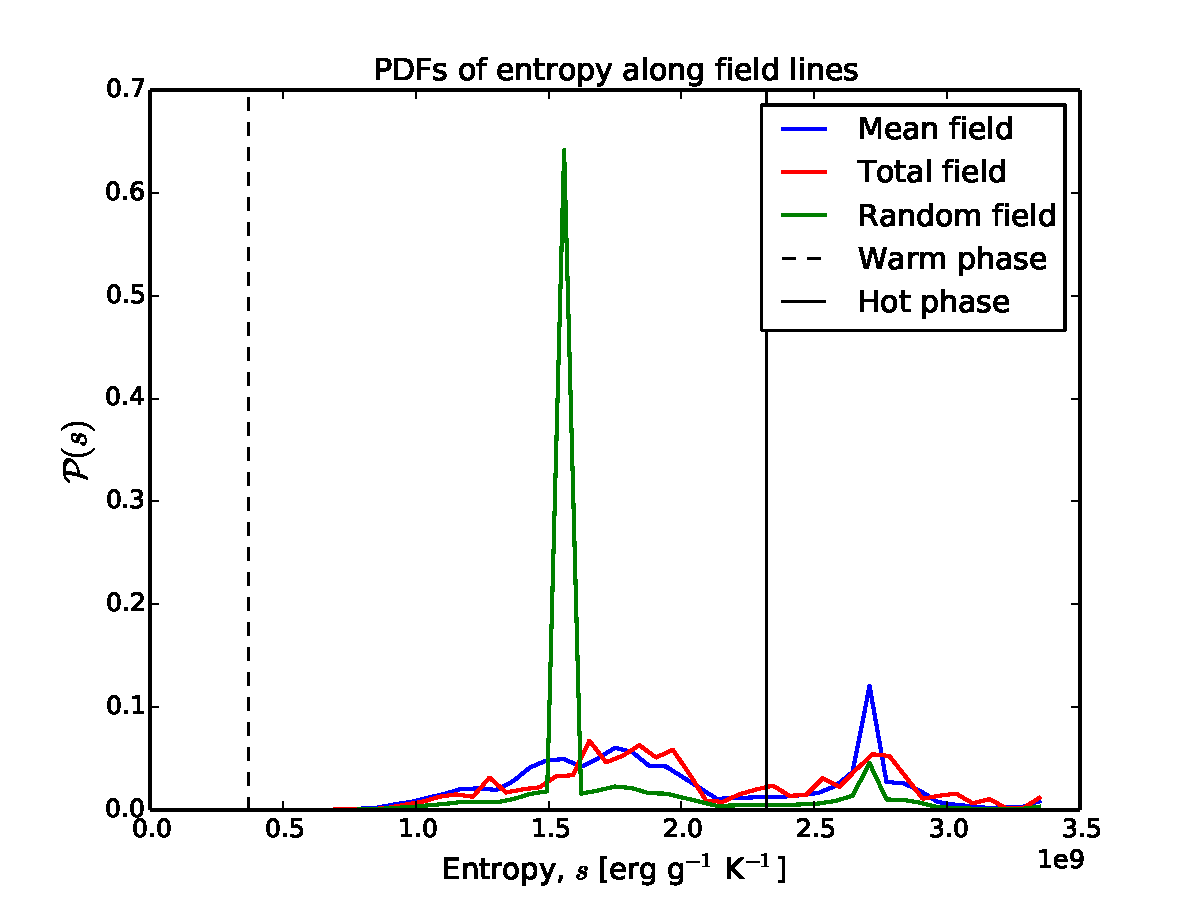
\includegraphics[width=\linewidth]{decomp_pdf_overall.pdf}
\caption{PDFs of $s$ along field lines of the mean (blue solid), total (red solid) and random (green solid) fields. The boundaries of between the cold and warm phases (black dashed) and between the warm and hot phases (black solid) are indicated.}
\label{fig:tot_pdfs}
\end{figure}
Figure \vref{fig:tot_pdfs} shows these PDFs. FIrstly, we note that all of the PDFs are clustered in the warm and hot phases. However, this is inextricably linked to the fractional volumes of the phases. It is difficult to discuss whether avoidance of the cold phase by the field line is also a contributing factor.\\
We concentrate on the warm and hot phases. The PDF for the total field is similar to that of the mean field in the warm phase. They both have a smooth distribution, even though the PDF of the total appears to be slightly more skewed. In the hot phase, the PDF for the total field is smooth. However, The PDF of the mean field peaks sharply, at approximately $s=27\cdot10^8$ erg g$^{-1}$ K$^{-1}$. Even though the PDF for the total field is smooth, its local maxima is close to this value of $s$. A similarly sharp peak is observed in this region for the PDF of the random field. This could suggest that $s=27\cdot10^8$ erg g$^{-1}$ K$^{-1}$ is a characteristic entropy associated with the hot phase for this snapshot. \\
A sharp peak is also observed in the warm phase in the PDF for the random field, at approximately $s=15.5\cdot10^8$ erg g$^{-1}$ K$^{-1}$. The probability density for the random field is weak outside of the sharp regions. It appears that the random field is characterised by a small range of entropy values in the warm and hot phases. 
\subsection{Curve fitting for PDFs of entropy}

 
\section{Conclusions}
%FAG
Note, that the mean magnetic field is strongest in the warm phase and the 
dynamo is strongest in the SN dense region within 500\pc of the midplane. 
These results support the hypothesis that the mean field is closely aligned to 
the warm phase of the ISM.
The fluctuating magnetic field is present in similar magnitude in all phases.
Note, in the warm phase, away from the midplane the magnetic field has a 
stronger vertical component, even though in these models the periodic boundary
conditions constrain the net $B_z$ to be zero on each horizontal slice. 
Given more open horizontal boundaries, we could anticipate the mean field 
actually to exhibit more vertical structure. 
With higher numerical diffusion required for the hot gas, the fluctuation 
dynamo in this phase may have been relatively suppressed, although the 
Reynolds numbers may have been higher than in the warm gas as both the length
scales and the velocities of the turbulence are tyically higher in the hot gas
than in the warm.
Nevertheless, a higher resolution run would be helpful in assessing how robust
is the alignment of the mean field to the warm phase, and whether the
fluctuating field in the hot phase may yet have relatively greater amplitude
than obtained here.
Given the dominance of the dynamo about the midplane, this may be feasible
without extending the domain vertically.

%end FAG

\newpage
\section*{Acknowledgements}

%FAG now moot
%CCE thanks Dr Frederick Gent for helpful discussions of his work.
%end FAG

%FAG include bibliography file refs.bib and amended cite codes 
%\begin{thebibliography}{99}
%\bibitem[\protect\citeauthoryear{Gent \textsl{et al}}{2013}]{GSFSM13} Gent F.A., Shukurov A., Sarson G.R., Fletcher A., Mantere M.J., 2012, MNRAS, 432, 1396-1423
%\bibitem[\protect\citeauthoryear{Gent \textsl{et al}}{2012}]{GSSFM13} Gent F.A., Shukurov A., Sarson G.R., Fletcher A., Mantere M.J., 2012, MNRASL
%\bibitem[\protect\citeauthoryear{Tennekes and Lumley}{1972}]{TL72} Tennekes H.,~Lumley J.L.,\emph{A First Course in Turbulence},~1972,~MIT Press
%\bibitem[\protect\citeauthoryear{Gent}{2012}]{Gent12} Gent F.A.,~PhD Thesis:~\emph{Supernova Driven Turbulence in the Interstellar Medium} ,~2012,~Newcastle University School of Mathematics and Statistics%,\url{<http://hdl.handle.net/10443/1755
%<http://hdl.handle.net/10443/1755>}
%\bibitem[\protect\citeauthoryear{Stepanov \textsl{et al}}{2002}]{SSFS02} Stepanov R.,~Frick P.,~Shukurov A.,~Sokoloff D.,~\emph{Wavelet tomography of the Galactic magnetic field},~2002,~A\&A,~391,~361-368
%\bibitem[\protect\citeauthoryear{Baddeley and Jensen}{2005}]{BJ04} Baddeley A.,~Jensen E.B.,~\emph{Stereology for Statisticians},~2005,~Chapman \& Hall/CRC
%\end{thebibliography}
  \bibliographystyle{mn2e}      % basic style, author-year citations
  \bibliography{refs}
% name your BibTeX data base
  \label{lastpage}
%end FAG

%\appendix

%\section[]{Large gaps in L\lowercase{y}${\balpha}$ forests\\* due to fluctuations in line distribution}

%(This appendix was not part of the original paper by
%A.V.~Raveendran and is included here just for illustrative
%purposes. The references are not relevant to the text of the
%appendix, they are references from the bibliography used to
%illustrate text before and after citations.)

%Spectroscopic observations of bright quasars show that the mean
%number density of Ly$\alpha$ forest lines, which satisfy certain
%criteria, evolves like $\rmn{d}N/\rmn{d}z=A(1+z)^\gamma$, where
%$A$ and~$\gamma$ are two constants.  Given the above intrinsic
%line distribution we examine the probability of finding large gaps
%in the Ly$\alpha$ forests.  We concentrate here only on the
%statistics and neglect all observational complications such as the
%line blending effect \citep[see][for example]{b11}.

%Suppose we have observed a Ly$\alpha$ forest between redshifts $z_1$
%and~$z_2$ and found $N-1$ lines.  For high-redshift quasars $z_2$~is
%usually the emission redshift $z_{\rmn{em}}$ and $z_1$ is set to
%$(\lambda_{\rmn{Ly}\beta}/\lambda_{\rmn{Ly}\alpha})(1+z_{\rmn{em}})=0.844
%(1+z_{\rmn{em}})$ to avoid contamination by Ly$\beta$ lines.  We
%want to know whether the largest gaps observed in the forest are
%significantly inconsistent with the above line distribution.  To do
%this we introduce a new variable~$x$:
%

\label{lastpage}

\end{document}
